\documentclass[manuscript, review, anonymous]{acmart}
%%
%% \BibTeX command to typeset BibTeX logo in the docs
\AtBeginDocument{%
  \providecommand\BibTeX{{%
    Bib\TeX}}}




\usepackage{xcolor}
% package for grey-out text box
\usepackage{tcolorbox}
% for table of recs (to merge rows)
\usepackage{multirow}
% to reference sections between documents
\usepackage{xr}
\usepackage{graphicx}
\usepackage{subcaption} % for images



\newcommand{\todo}[1]{\textcolor{red}{[TODO: #1]}}
\newcommand{\alice}[1]{\textcolor{orange}{[Alice: #1]}}


\usepackage{titlesec}
\usepackage{enumitem}

\usepackage{longtable}
\usepackage{subcaption}
\usepackage{multirow}



\newcommand{\orgs}[0]{\textbf{Organizations~}}
\newcommand{\teams}[0]{\textbf{Teams~}}
\newcommand{\inds}[0]{\textbf{Individuals~}}
% \newcommand{\recommendation}[1]{\paragraph{\textit{#1}}}

\newcommand{\recsection}[3]{
    \paragraph{\textit{#1}} {#2}
    \ifthenelse{\equal{#3}{}}{}{\newline\hspace*{2em}\textit{Consider}: #3}
}

\renewcommand{\sectionautorefname}{Section}
\renewcommand{\subsectionautorefname}{Section}
\renewcommand{\subsubsectionautorefname}{Section}
\renewcommand{\figureautorefname}{Figure}

% fixing issues with whitespace
\hyphenpenalty=10000
\brokenpenalty=10000
\sloppy
\raggedbottom



\begin{document}

\title[]{}


\author{Alice Qian}
\email{aqzhang@andrew.cmu.edu}
\affiliation{%
  \institution{Carnegie Mellon University}
  \state{Pennsylvania}
  \country{USA}
}
\author{Ziqi Yang}
\email{ziqiyang@andrew.cmu.edu}
\affiliation{
    \institution{Carnegie Mellon University}
    \state{Pennsylvania}
    \country{USA}
}


\author{Ryland Shaw}
\orcid{0009-0008-6123-1781}
\email{v-rylandshaw@microsoft.com}
\affiliation{%
  \institution{Microsoft Research}
  \city{New York City}
  \state{New York}
  \country{United States}
}


% TO DO 
\author{Jina Suh}
\email{jinsuh@microsoft.com}
\affiliation{%
  \institution{Microsoft Research}
  \country{USA}}

      
\author{Laura Dabbish}
\email{dabbish@andrew.cmu.edu}
\affiliation{%
  \institution{Carnegie Mellon University}
  \country{USA}}

  
\author{Hong Shen}
\email{hongs@andrew.cmu.edu}
\affiliation{%
  \institution{Carnegie Mellon University}
  \country{USA}}





  \begin{CCSXML}
<ccs2012>
   <concept>
       <concept_id>10003120.10003121.10003129</concept_id>
       <concept_desc>Human-centered computing~Interactive systems and tools</concept_desc>
       <concept_significance>500</concept_significance>
       </concept>
   <concept>
       <concept_id>10010147.10010178</concept_id>
       <concept_desc>Computing methodologies~Artificial intelligence</concept_desc>
       <concept_significance>500</concept_significance>
       </concept>
   <concept>
       <concept_id>10003120.10003121.10011748</concept_id>
       <concept_desc>Human-centered computing~Empirical studies in HCI</concept_desc>
       <concept_significance>500</concept_significance>
       </concept>
   <concept>
       <concept_id>10003120.10003130.10011762</concept_id>
       <concept_desc>Human-centered computing~Empirical studies in collaborative and social computing</concept_desc>
       <concept_significance>500</concept_significance>
       </concept>
   <concept>
       <concept_id>10003456.10003462</concept_id>
       <concept_desc>Social and professional topics~Computing / technology policy</concept_desc>
       <concept_significance>500</concept_significance>
       </concept>
 </ccs2012>
\end{CCSXML}

\ccsdesc[500]{Human-centered computing~Interactive systems and tools}
\ccsdesc[500]{Computing methodologies~Artificial intelligence}
\ccsdesc[500]{Human-centered computing~Empirical studies in HCI}
\ccsdesc[500]{Human-centered computing~Empirical studies in collaborative and social computing}
\ccsdesc[500]{Social and professional topics~Computing / technology policy}


\renewcommand{\shortauthors}{Alice Qian Zhang, et al.}

\begin{abstract}
Responsible AI (RAI) content work, such as annotation, moderation, or red teaming for AI safety, often exposes crowd workers to potentially harmful content. While prior work has underscored the importance of communicating well-being risk to employed content moderators, designing effective disclosure mechanisms for crowd workers while balancing worker protection with the needs of task designers and platforms remains largely unexamined. To address this gap, we conducted co-design sessions with 29 task designers, workers, and platform representatives. We investigated task designer preferences for support in disclosing tasks, worker preferences for receiving risk disclosure warnings, and how platform stakeholders envision their role in shaping risk disclosure practices. We identify \todo{change this part here since the dimensions aren't a key finding} key design tensions around specificity, worker agency, and task designer responsibility, and map the socio-technical tradeoffs that shape disclosure practices. We contribute design recommendations and feature concepts for risk disclosure mechanisms in the context of RAI content work. 
\end{abstract}



%  TO DO add ccs

%%
%% Keywords. The author(s) should pick words that accurately describe
%% the work being presented. Separate the keywords with commas.
\keywords{Responsible AI, crowdsourcing, well-being, data work, red teaming, RAI content work}
% \received{January 2024}
% \received[revised]{July 2024}
% \received[accepted]{October 2024}

%%
%% This command processes the author and affiliation and title
%% information and builds the first part of the formatted document.
% \title{Canary in the Digital Coal Mine: Co-designing Psychological Risk Communication for RAI Content Work}
% Disclosing Risk, Negotiating Harm: Cross-Stakeholder Design of Task Warnings
% Translating Harm: Designing Severity Disclosures Across Stakeholders
% Co-Designing Harm Disclosure: A Multi-Stakeholder Approach to Risk in Crowdwork
\title[Worker Discretion Advised]{Worker Discretion Advised: Co-designing Risk Disclosure in Crowdsourced Responsible AI (RAI) Content Work}

% \title{Navigating Risk and Responsibility in AI Task Design}
% title options: RISE (Risk-Informed, Safe, and Ethical AI Task Design), RAID (Risk Accountability in AI Design), Foundations for Safe AI Task Design, Navigating AI Risks: A Framework for Responsible Task Design, Responsible AI Task Design, Balancing Act: Safe and Responsible AI Task Design
\maketitle

\section{Introduction}

% SECTION 1: What is the problem? Why is it important?
\textbf{Responsible AI (RAI) content work} ~\cite{qian2025aura}, such as annotation, moderation, and red teaming of AI systems for safety, has become essential as organizations grapple with the risks of increasingly powerful AI systems. The rapid expansion of Generative AI (GenAI) has only heightened this reliance, fueling demand for large-scale human oversight to detect and mitigate safety concerns \cite{StanfordHAI2025AIIndex, GrandViewResearch2024GenerativeAI}. %As organizations invest more heavily in safety measures, RAI content work becomes increasingly essential to help in the training and evaluation of AI systems for potential risks~\cite{udupa2023ethical}. 
Meeting this demand, however, requires human labor to confront harmful material ranging from explicit violence and hate speech to more subtle forms of bias and manipulation that demand nuanced human judgment~\cite{qian2025aura}. Such exposure can cause significant psychological distress, and researchers have documented its toll on both part-time and full-time RAI workers~\cite{roberts2016commercial, qian2025aura}, including burnout, anxiety, depression, and in extreme cases post-traumatic stress disorder (PTSD)~\cite{alemadi2024emotional, martinez2024secondary, spence2025content, gebrekidan2024content}.


Increasingly, organizations externalize RAI content work to \textbf{crowdsourcing platforms}, or platforms that outsource jobs \textit{``to an undefined, generally large group of people through the form of an open call''} ~\cite{howe2006rise, berg2018digital}. These platforms provide the infrastructure for on-demand, distributed labor markets, which AI companies then leverage to scale annotation, moderation, and adversarial testing \cite{udupa2023ethical, mann2025meta, egelman2014crowdsourcing}.
\textbf{Crowdworkers}~\cite{berg2018digital} may face significant \textbf{well-being risks} when taking on tasks that involve graphic violence, disturbing imagery, or to simulate harmful scenarios designed to probe AI system boundaries~\cite{qian2025locating}. 
Unlike part-time or full-time employees in traditional RAI roles, who may receive institutional support such as mental health support or training ~\cite{qian2025aura, roberts2016commercial, steiger_psychological_2021}, crowdworkers often perform this work in isolation, without adequate preparation or access to support systems ~\cite{schlicher2021flexible, berastegui2021exposure}. 


% SECTION 2: what's been tried/why it didn't work
% existing risk disclsoure and transparency efforts in crowdsourcing
Past work in HCI and CSCW has extensively examined the structural condition of crowd work ~\cite{gray2016crowd, silberman2018responsible,salehi2015we}. In particular, foundational efforts like Turkopticon sought to increase transparency by surfacing requester reputations~\cite{irani2013turkopticon}, yet few platform-embedded mechanisms exist to help workers anticipate or avoid emotionally distressing or harmful tasks. In fact, platforms vary widely in their practices, from providing no disclosure options to offering more structured resources ~\cite{prolific2025participant, prolific2025sensitive, ProlificAPIContentWarning2025}. At the same time, prior research has advanced content warnings for social media audiences~\cite{Zhang2024PerceptionsTriggerWarnings, shashirekha2023trigger, bell2025warning}, but it remains unclear how to adapt these insights to workers facing risk disclosure in crowdsourced RAI tasks. Despite growing awareness of well-being risks -- especially in RAI content work -- there is little empirical research on how these risks are communicated and how disclosure practice might be improved. This gap underscores the need to examine \textbf{``risk disclosure''} -- the provision of upfront information about the
nature and potential harms of content tasks ~\cite{bharucha2023content, qian2025aura} -- not merely as an ethical responsibility, but as a ``design challenge'' embedded within sociotechnical systems that often obscure harm.

%Current approaches to informing potential crowdworkers about the risks of RAI content work lack grounding in an empirical understanding of stakeholder needs across the crowdsourcing ecosystem. Platforms vary widely in their practices, from providing no disclosure options to offering more structured resources ~\cite{prolific2025participant, prolific2025sensitive, ProlificAPIContentWarning2025}. Moreover, prior research has established that the burden of disclosing risks is disproportionately placed on the \textbf{task designers} or \textit{``individuals who design and post RAI content work tasks''}~\cite{qian2025locating}. Even when platforms present more options for risk disclosure, little evidence shows that these mechanisms account for the perspectives of task designers and workers, the stakeholders most directly affected. Lessons from prior research that incorporates the perspectives of workers in designing interventions on crowdsourcing platforms have demonstrated the benefits of taking collaborative-design approaches~\cite{irani2016stories, mturk2018aup, silberman2018responsible}.

%Despite the critical role of crowdworkers workers in RAI, the lack of adequate risk disclosure is exacerbated by the omission of worker well-being in most AI transparency frameworks designed to promote ethical AI development. Model cards~\cite{mitchell2019model}, datasheets~\cite{gebru2021datasheets}, and crowdworksheets~\cite{diaz2022crowdworksheets} set important precedents for documenting technical specifications and data collection processes~\cite{gebru2021datasheets, diaz2022crowdworksheets, mitchell2019model}, yet they primarily focus on model performance and bias, often overlooking the immediate welfare of workers involved in data creation and evaluation. This reveals a significant gap in tools for ethical AI development--between technical transparency, which documents what models do, and worker protection transparency, which should inform content workers about the risk they face~\cite{bharucha2023content}. The result is a disconnect between the growing establishment of AI transparency tools and the minimum safety information needed by workers who make safe AI development possible. 

Such a ``design challenge'' is further complicated by the inherent tension between stakeholder needs and incentives ~\cite{finnerty2013keep, gaikwad2016boomerang, salehi2015we, irani2013turkopticon, salehi2018ink}. Prior work has revealed that task designers\footnote{We use the term \textbf{task designers} rather than requesters to more accurately reflect the active and interpretive role individuals play in shaping the structure, framing, and content of crowdsourcing tasks. While requester is the platform-standard term, it implies a transactional relationship that downplays the design decisions and ethical considerations embedded in task creation. Following prior HCI work that emphasizes the creative and normative dimensions of task design~\cite{bragg2018sprout, qian2025locating}, we adopt task designer to foreground their agency and responsibility in shaping worker experience.} face pressure to recruit sufficient workers while also meeting ethical obligations to inform them of potential risks~\cite{qian2025locating, finnerty2013keep, kittur2008crowdsourcing, zheng2011task, bragg2018sprout}, while workers need agency to make informed participant decisions and fair compensation for their labor~\cite{irani2013turkopticon, salehi2018ink, martin2014being, silberman2018responsible, toxtli2021quantifying, schlicher2021flexible}, and platforms must balance worker safety with operational efficiency and legal compliance~\cite{gaikwad2016boomerang, xu2017incentivizing, xia2020privacy, allen2018design}. 
As Fieseler et al ~\cite{fieseler_unfairness_2019} remind us, crowdsourcing platforms mediate a triadic relationship between requester, worker, and platform, yet much of the existing literature focuses only on a dyadic exchange between workers and task designers.
To navigate these tradeoffs, it is therefore critical to examine the unique tensions faced by the three main stakeholders in crowd-based RAI content work -- task designers, workers, and platform -- and to offer guidance that supports ethically grounded decisions aimed at promoting worker well-being. Our aim is to complement worker-centered scholarship by concentrating on the actors who currently shape task structure, disclosure policy, and enforcement.
% Previous research has shown that of the three types of actors in this relationship, workers hold the least decision making power for this reason, we hope to include all three perspectives to have a clear understanding of design opportunities given tensions among all three stakheolders. \todo{add just 1 sentence here about why we are not centering workers' perspective, in case we get some critical reviewers}

% SECTION 3: what's new with our approach (why it is great :))
To address this gap, we conducted one-on-one co-design sessions \cite{tang2024ai,kuo2023understanding} with 15 task designers, 11 workers, and 3 platform representatives to understand how risk disclosure decisions are made and what tools and workflows could better support effective disclosure practices. Our study focused on three key design dimensions: specificity (how detailed or granular the disclosure is), worker agency (the extent to which workers can act on disclosure), and task designer agency (the flexibility and support available to those creating disclosures). We ask the following research questions:\textbf{\textit{ RQ1:}} How do task designers, workers, and platform representatives perceive and approach different risk disclosure mechanisms across key design dimensions? and \textbf{\textit{RQ2: }}What tradeoffs and tensions emerge when stakeholders consider different configurations of risk disclosure mechanisms?  
%\begin{enumerate}
%  \item How do task designers, workers, and platform representatives perceive and approach different risk disclosure mechanisms across key design dimensions? 
 % \item What tradeoffs and tensions emerge when stakeholders consider different configurations of risk disclosure mechanisms?  
%\end{enumerate}

%Co-design methodology offers a particularly valuable approach for this challenge because it allows us to understand the complex constraints and considerations that shape each individual's perspective while collaboratively exploring solutions that can work for their specific role. By engaging in individual co-design sessions with task designers who use disclosure mechanisms, workers who must interpret and act on disclosure information, and platform representatives who implement and govern these systems, our study captures the full complexities of risk disclosure as a sociotechnical challenge that spans individual and platform levels. 

%Our workshops engaged participants in systematically evaluating risk disclosure mechanisms across three key design dimensions: (1) \textbf{Specificity}: ranging from binary warnings to content type categorization to specific content examples; (2) \textbf{Worker agency}: from no opt-out options to informed consent to granular control over exposure levels; and (3) \textbf{Task designer agency}: from generic disclosure templates to manual customization to AI-based disclosure recommendations. Our decision to focus on these dimensions has been informed by prior research on content warnings on social media platforms~\cite {Zhang2024PerceptionsTriggerWarnings, vit2025use} and on the importance of incorporating perspectives of workers~\cite{salehi2018ink,salehi2015we} and task designers~\cite{qian2025locating, gutheim2012fantasktic, bragg2018sprout} in platform interventions. 

Our findings reveal that workers, task designers, and platforms hold divergent expectations about how risk should be communicated in RAI content work. Workers value clear, specific warnings and the ability to make informed decisions; task designers often fear that detailed disclosures will deter participation; and platforms aim to balance protection with policy and scalability. These tensions manifest across key stages of task engagement -- from sign-up and participation to post-task feedback -- and expose structural gaps in responsibility. We identify design opportunities to better support disclosure practices, including adaptive filters, feedback mechanisms, and AI-assisted tools. Ultimately, we argue that risk disclosure is not just a technical feature but a sociotechnical negotiation of power, protection, and participation. We also acknowledge the limits of co-design in this space, and that some categories of RAI content work should not be crowdsourced, in which case it may be better to redesign the pipeline for gathering worker input rather than the disclosure itself.
% \todo{add just one sentence here to preemptive talk about limitations of co-design, what type of RAI work should not be crowdsourced (our 5.4).}
% Our multi-stakeholder methodology represents one of the first empirical investigations of risk disclosure design considerations for RAI content work, contributing novel insights into how the intersection of AI development needs, platform constraints, worker protection concerns, and regulatory pressures shapes the disclosure ecosystem in this critical but understudied domain. Through analysis of our co-design session findings, we contribute a multi-stakeholder understanding of risk disclosure in crowdsourced RAI content work, surfacing core tensions across workers, task designers, and platforms, and offering design implications for more accountable and transparent worker protection.

Our contributions are threefold:

\begin{itemize}
\item \textbf{Empirical insights} into risk disclosure in crowdsourced RAI content work, based on co-design sessions with 15 task designers, 11 workers, and 3 platform representatives. We surface how stakeholder roles, values, and constraints shape disclosure expectations and practices.
\item \textbf{A multi-stakeholder understanding} of risk disclosure as a sociotechnical negotiation, identifying key tensions around specificity, worker agency, and task designer responsibility across the lifecycle of content tasks.
\item \textbf{Design implications} for more accountable and transparent disclosure systems.

\end{itemize}

\section{Related Work}
\begin{figure}
  \centering
  \includegraphics[width=0.6\linewidth]{figures/mturk_adult_qualification.pdf}
  \caption{MTurk’s adult content qualification requirement for screening workers.}
  \label{fig:mturk_adult}
\end{figure}


\begin{figure}
  \centering
  \begin{subfigure}[b]{0.48\linewidth}
    \centering
    \includegraphics[width=\linewidth]{figures/prolific_zoomedin_binary.pdf}
    \caption{Close-up of the sensitive content warning presented to workers.}
    \label{fig:prolific_zoomed}
  \end{subfigure}
  \hfill
  \begin{subfigure}[b]{0.48\linewidth}
    \centering
    \includegraphics[width=\linewidth]{figures/prolific_worker_side_example.pdf}
    \caption{Worker-facing task list view with a sensitive content label.}
    \label{fig:prolific_worker}
  \end{subfigure}
  \caption{Prolific’s interface-level disclosure mechanisms from the worker perspective.}
  \label{fig:prolific_worker_pair}
\end{figure}

\begin{figure}
  \centering
  \includegraphics[width=\linewidth]{figures/warning_zooniverse.pdf}
  \caption{Task content warning from Zooniverse}
  \label{fig:zooniverse_removed}
\end{figure}

\begin{figure}
  \centering
  \includegraphics[width=0.7\linewidth]{figures/toloka_removed_task.pdf}
  \caption{Removed task page from Toloka, demonstrating limited access to past sensitive content.}
  \label{fig:toloka_removed}
\end{figure}


%\subsection{Risk Disclosure and Transparency in Crowdsourcing}
\subsection{Psychological and Well-being Risks of RAI Content Work} 
The rise of Responsible AI (RAI) initiatives draws new attention to the people behind the systems: workers who annotate, moderate, and evaluate AI content. These tasks -- collectively described as \textit{Responsible AI (RAI) content work} \cite{qian2025aura}, including annotation, moderation, and red teaming for model safety -- are critical to system performance and societal impact. Yet the labor remain largely invisible or undervalued ~\cite{gray2019ghost}. 

In particular, a growing body of research has documented the \textit{psychological and well-being risks} faced by these workers. Workers involved in those RAI content work routinely experience graphic or disturbing material with significant negative mental-health effects.  Studies show that prolonged exposure coupled with limited support contributes to burnout ~\cite{dosono2019moderation}, secondary trauma ~\cite{martinez2024secondary}, and PTSD ~\cite{steiger_psychological_2021, alemadi2024emotional, Michel2018ExContentMS, ruckenstein_re-humanizing_2020, Dwoskin_2019, arsht_2018_human}. More recent work replicates these findings, reporting that a large portion of content moderators exhibit moderate to severe psychological distress and low well-being \cite{Spence2025ContentModeratorMentalHealth}. Other research highlights broader harms, including privacy violations~\cite{pinchevski2023social, schopke-gonzalez_why_2022} and changes in workers’ personal beliefs and moral outlooks~\cite{newton_trauma_2019, Stackpole_2022, Douek_2021}.
%However, given the rapidly evolving nature of AI data work and limited investigation of employment contexts such as crowdsourcing, there is a pressing need to better understand the experiences, needs, and challenges of workers in these environments.

These well-being risks are compounded by the lack of support structures. While researchers are beginning to explore how organizations and individuals with decision-making power may support and address these psychological and well-being risks~\cite{qian2025aura, qian2025locating, steiger_psychological_2021, bharucha2023content}, most of this work has focused on full-time employees in formal moderation roles. Far less is known about how crowdworkers --- who perform similar tasks under more precarious conditions --- encounter and navigate these risks, which is the focus of this study.


\subsection{Risk Disclosure in Crowdsourcing Platform: A Multi-Stakeholder Challenge}
Although risk disclosure is recommended as a key practice to support worker well-being in RAI content work~\cite{bharucha2023content, qian2025aura}, it has primarily been discussed in the context of full-time employment and platform-based content moderation. This is a significant gap, as crowdworkers increasingly perform similar high-risk annotation and moderation tasks, often with little to no warning about potentially graphic or disturbing content, such as depictions of violence, self-harm, or abuse. These workers operate in task-based gig economies where formal protections like HR support or institutional mental health resources are typically absent~\cite{irani2013turkopticon, martin2014being, salehi2018ink, silberman2018responsible, toxtli2021quantifying, schlicher2021flexible}.

%be exposed to graphic or disturbing content, such as depictions of violence, self-harm, or abuse, without prior warning or support infrastructure. Unlike traditional employees, these workers often operate in task-based gig economies where formal HR policies or worker protections are absent~\cite{irani2013turkopticon, salehi2018ink, martin2014being, silberman2018responsible, toxtli2021quantifying, schlicher2021flexible}. As a result, the mechanisms and norms for disclosing potential harms in job postings or task instructions are highly variable.

%While prior literature has examined the psychological toll of content moderation specifically~\cite{spence2025content, alemadi2024emotional, steiger_psychological_2021}, which entails exposure to similarly harmful content as RAI content work \cite{qian2025aura, gillespie2025airedteamingsociotechnicalchallenge}, there is limited work describing how task-level risk information is communicated to annotators in crowdsourced settings. In this study, we investigate how risk should be disclosed in job ads and instructions for RAI content work tasks on crowdsourced work platforms. Our aim is to understand how task designers, workers, and platform representatives navigate risk disclosure mechanisms and the design tensions that emerge from tradeoffs shaping their disclosure decisions.
%\subsubsection{Risk Disclosure for Part-Time and Full-Time Jobs}

While prior HCI and CSCW work has extensively investigated the structural dimensions of crowdsourcing platforms, much of it has yet to address how well-being risks are communicated, managed, or shared. %  how crowdsourcing platforms are sites of recurring tension, where the balance among labor, automation, and governance is contested<CITES>. Platforms mediate a ``triadic relationship'' among workers, task designers, and the platform \cite{fieseler_unfairness_2019}. 
Foundational work by Irani et al. introduced Turkopticon, a system that surfaced worker–requester power asymmetries and challenged the opaque design of Amazon Mechanical Turk~\cite{irani2013turkopticon}. Following this, researchers have explored how platforms mediate relationships through design, algorithms, and incentives. Trade-offs between efficiency and fairness are deeply embedded in task workflows, reward structures, and rating systems~\cite{ho2015incentivizing}. Beyond facilitating labor, these systems act as sociotechnical infrastructures in which institutional values are deeply inscribed.
%Crowdsourcing acts as a sociotechnical infrastructure where values are encoded into design <CITES>.

From the worker's perspective, platform design can constrain or enable agency, but rarely centers on well-being. While crowdsourcing is often framed as flexible or empowering, studies show that this flexibility is unevenly distributed and often illusory~\cite{rechkemmer2022understanding, varanasi2022feeling, liang2021embracing}. Workers face well-documented challenges with task rejections~\cite{mcinnis2016taking}, opaque reputation mechanisms~\cite{saito2019turkscanner}, and emotional strain~\cite{flores2020challenges, martin2014being}, especially in tasks involving harmful or triggering content.

For task designers, the dominant focus is data quality, throughput, and consistency. However, recent work argues to re-examine how task designers might reflect on their interpretive and creative agency in shaping task content, instructions, and interaction dynamics~\cite{zheng2011task, bragg2018sprout, qian2025locating}. Studies have shown how task design choices --- including instruction clarity~\cite{wu2017confusing}, interface affordances~\cite{han2020crowd}, and incentive structures~\cite{ho2015incentivizing} --- can significantly influence worker outcomes. Calls for greater transparency in task designer identity and intention aim to help workers make more informed decisions and reduce asymmetries in trust and accountability~\cite{sutherland2018sharing, whiting2019fair, qian2025locating}.

At the platform level, governance practices shape how risk is managed, but often opaquely. Platforms mediate access to tasks, set rules, and enforce labor norms, but workers and task designers alike have limited visibility into these processes~\cite{toxtli2021quantifying, whiting2019fair, fieseler_unfairness_2019}. Algorithmic interventions, automated quality checks, and visibility constraints are not neutral; instead, they structure who gets to work, under what conditions, and with what recourse~\cite{gadiraju2017modus, rzeszotarski2012crowdscape}. While some platforms have introduced features aimed at promoting fairness and accountability~\cite{silberman2018responsible, whiting2019fair}, many continue to obscure institutional priorities behind claims of neutrality and scale~\cite{gray2016crowd, kingsley2015accounting}.

Yet despite these structural dynamics, little is known about how these stakeholders involved in RAI content work actually perceive, interpret, and implement risk disclosure in practice. Prior work has not examined how disclosure responsibilities are negotiated across roles, or what trade-offs shape real-world decisions. This paper addresses the gap by examining how task designers, workers, and platform representatives approach risk disclosure in crowdsourced RAI tasks. Through a multi-stakeholder investigation, we surface the tensions, frictions, and opportunities that shape disclosure practices, laying the groundwork for more transparent, protective, and equitable design.

\subsection{Risk Disclosure as a Design Challenge}
While academic and organizational discourse has increasingly underscored the importance of disclosing well-being risks in RAI content work, particularly for employed roles such as content moderators~\cite{bharucha2023content, qian2025locating}, less is known about how such efforts are operationalized in crowdsourcing contexts. %In particular, it remains unclear how workers and task designers perceive existing platform features intended to support disclosure, how those features function in practice, and what alternative designs should be explored.

%Task designers often lack structured guidance for implementing content warnings or consent flows in the task specification stage for RAI content work tasks~\cite{qian2025locating}. 

On the one hand, most crowdsourcing platforms offer limited, inconsistent, or opaque mechanisms for risk disclosure. % or ensuring their adoption when they do exist. One approach is allowing task designers to specify in different ways that their task contains sensitive content. 
Prolific, for example, provides a researcher-facing ``sensitive content'' toggle during study design (Figure \ref{fig:prolific_zoomed} along with an option to include additional information with keywords (see Figure \ref{fig:prolific_keywords}, along with guidelines to include warnings in task descriptions for both task designers ~\cite{ProlificResearcherSensitive2025, ProlificAPIContentWarning2025} and workers~\cite{prolific2025participant}. Another approach is to limit exposure based on age limits or other qualifications. Amazon Mechanical Turk (MTurk), for example, provides task designers with an ``adult content qualification'' requirement option in which only workers who have received this certification can see tasks with such content (see Figure \ref{fig:mturk_adult}). Research platforms such as Zooniverse and Tokola provide examples of task-level warnings (see Figure \ref{fig:zooniverse_removed} and Figure \ref{fig:toloka_removed}), but these remain inconsistent in format and enforcement.
%Platforms such as DataAnnotation, Remotasks, and SurgeAI, lock their interfaces behind employment verification systems, and publicly available information about their risk disclosure process is scarce. Platforms used for crowdsourced research, such as Zooniverse and Tokola, have documented similar types of warnings for tasks (see Figure \ref{fig:zooniverse_removed}).  At the surface level we see a lack of consensus across platforms around how risk disclosure should be supported within crowdsourcing infrastructures.
Beyond disclosure options, platform-level governance also varies significantly. %Platforms have the power to moderate or enforce risk disclosures. There is limited publicly available documentation, however, on how platforms make decisions on what tasks or content are permitted. 
For example, Prolific allows workers to report tasks for review and potential removal, and anecdotal evidence suggests platforms like Toloka have occasionally removed tasks after worker complaints (Figure~\ref{fig:toloka_removed}). However, such interventions appear to be the exception rather than the norm.

On the other hand, past work on content warnings on consumer-facing platforms offers important lessons for designing risk disclosures for RAI work. Social media platforms such as Tumblr, Twitter (now X), Instagram, and TikTok have implemented content warnings to protect users from potentially distressing material, ranging from textual tags like \#tw to automated overlays that blur graphic images. These systems aim to support informed consent, reduce harm, and signal sensitivity to trauma~\cite{Zhang2024PerceptionsTriggerWarnings, vit2025use}. However, their application is highly variable and their effectiveness remains contested. Empirical studies show that while users generally appreciate warnings in principle, concerns persist about inconsistent enforcement, insufficient granularity, and unclear rationale~\cite{charles2022typology, bridgland2024meta, bell2025warning}. Some warnings may even increase anticipatory anxiety, especially among individuals with lived experience of trauma~\cite{sharevski2022meaningful}. These limitations highlight the complexity of operationalizing harm reduction at scale and suggest that risk disclosure is not simply a matter of adding labels, but requires careful design attuned to user needs, platform affordances, and sociocultural context.

More importantly, the context of crowdsourced RAI work differs in important ways. Unlike social media users, who encounter warnings during voluntary content consumption, crowdworkers engage with potentially harmful material as part of paid, high-throughput tasks. As such, risk disclosure in this domain intersects with distinct incentives -- such as performance expectations, compensation structures, and data quality requirements -- that reshape the meaning of consent, exposure, and protection. These differences raise critical questions about how content warning strategies must be re-imagined for labor systems, not simply adapted from consumer platforms.

In this study, we build on these insights to examine how risk disclosure is approached, interpreted, and contested in the context of crowdsourced RAI content work. We frame risk disclosure not as a compliance checkbox or content tag, but as a complex design challenge that must account for divergent stakeholder needs, uneven power relations, and structural gaps in responsibility and support.

%Overall, platform-level features for risk disclosure are inconsistent, unreliably enforced, and often rely on the initiative of individual task designers. Without formalized mechanisms for validation or enforcement, responsibility for ethical disclosure is effectively decentralized. This ambiguity raises critical questions about accountability and reveals how existing systems prioritize flexibility and throughput over standardized support. In this study, we examine how risk disclosure dynamics are navigated in practice by workers, task designers, and platforms alike and how current approaches reflect broader tensions between different stakeholder. %We conceptualize risk disclosure as a design space defined by timing of disclosure before or during or after a task, scope and granularity of information, control over gating and opt out, visibility to stakeholders, validation of claims, and enforcement mechanisms.


% Transparency tools such as model cards, datasheets and crowdworksheets document model behavior and data provenance but seldom address worker well-being; meanwhile, research on trigger and content warnings reveals the complexities of communicating risks to users.  Computational efforts aim to automatically assign trigger warnings to social media posts and fan-fiction \todo{citations}, but performance remains modest and the taxonomy of warnings is contested~\cite{Wiegmann2023Trigger}.  Bridgland et al.’s meta-analysis of trigger-warning experiments finds that warnings do not reduce distress and may increase anticipatory anxiety~\cite{Bridgland2024Meta}, highlighting the lack of consensus about their effectiveness.  Diaz et al.’s CrowdWorkSheets framework calls for documenting annotator demographics and decision points in data collection~\cite{Diaz2022CrowdWorkSheets}, while Turri et al.\ argue that existing transparency efforts focus on downstream users and overlook the needs of data creators and moderators~\cite{Turri2024Transparency}.  These findings support our claim that current tools fall short in communicating risks to workers and that empirically grounded disclosure mechanisms are needed.





%\subsection{Lessons from Content Warnings on Social Media Platforms}
%\todo{Add a brief review of research on warnings from human factors? like pre-internet research}
% from laura
% https://www.sciencedirect.com/science/article/pii/S0003687002000091?casa_token=PRWc3Ycbrj0AAAAA:pETsBivTstXdlz9obPRdNyFX8RKeZktc-OR7nvAxqvO1_kt0wJAwOS8lTglhAqzZoTAaXfsFdg#BIB99
% https://www.sciencedirect.com/science/article/pii/S0003687002000091?casa_token=PRWc3Ycbrj0AAAAA:pETsBivTstXdlz9obPRdNyFX8RKeZktc-OR7nvAxqvO1_kt0wJAwOS8lTglhAqzZoTAaXfsFdg
%Content warnings on social media platforms are an example of a platform-level intervention for communicating content risk. Digital content and trigger warnings (TWs/CWs) were originally developed by social media platforms as a mechanism to give users greater control over their exposure to distressing content. Platforms such as Tumblr, Twitter (now X), Instagram, and TikTok have increasingly relied on warnings to label content related to potentially disturbing topics such as self-harm, suicide, eating disorders, more. These warnings serve multiple purposes: protecting users’ psychological well-being, signaling platform sensitivity to trauma, and minimizing liability through proactive disclosure~\cite{Zhang2024PerceptionsTriggerWarnings, vit2025use}. Although these content warning systems represent risk communication design work, they've primarily been implemented in consumer-facing contexts rather than labor platforms.

%Content warnings appear in varied forms~\cite{charles2022typology}. Some are user-applied tags or hashtags (e.g., \#tw, \#cw), while others are system-generated overlays that blur images or restrict content with interstitial warnings such as ``sensitive content ahead.'' Warnings are often differentiated by modality: graphic video content might receive stricter AI-driven flags, whereas textual descriptions rely more on user discretion. The rationale behind these warnings can differ: some aim to reduce harm, others to promote informed consent or foster a respectful discourse environment~\cite{gomes2024problematizing}. This diversity reflects both the flexibility and inconsistency in how platforms define risk and empower users, raising questions about how such designs might or might not translate into the labor context.

% should probably add a figure somewhere here
%Although widely adopted, existing content warning systems are not without limitations. Despite their intentions, content warning systems remain contested~\cite{sharevski2022meaningful, vitak_beyond_2016}. Interviews with social media users show a broad consensus that warnings are helpful in principle, yet concerns persist around inconsistent application, limited nuance, and unclear guidelines for use~\cite{Zhang2024PerceptionsTriggerWarnings}. Some users expect systems to preemptively shield them from trauma, while others see warnings as overly cautious or stifling to expression. Empirical studies suggest that warnings often do little to reduce emotional distress and may even increase anticipatory anxiety, especially among individuals with relevant lived experience~\cite{bridgland2024meta, bell2025warning}. In practice, it remains a challenge to strike a balance between over-warning and under-warning in these systems, with the burden frequently falling on creators to self-disclose in the absence of clear platform guidance~\cite{vit2025use}. These shortcomings highlight the challenges of operationalizing harm reduction at scale, insights that are highly relevant to understanding risk disclosure mechanisms in crowdsourced labor environments.

% Content moderation policies vary significantly across social media platforms, and enforcement remains opaque and inconsistent~\cite{gomes2024problematizing, gibbs2015facebook}. Though the U.S. Surgeon General has called for warning labels to protect youth mental health (i.e., analogous to tobacco packaging warnings) these proposals remain politically and legally contested~\cite{murthy2024surgeon}. Such tensions between user expectations and platform enforcement underscore the difficulty of balancing protection, autonomy, and expression, dynamics that are equally salient in worker-facing systems. 

%Taken together, content warnings represent a growing, if imperfect, strategy for risk disclosure in digital environments. Yet despite their increasing adoption in consumer-facing media, few analogues exist for informing crowdworkers of potentially distressing material. Understanding how labor-specific practices diverge from social media conventions is critical for designing effective and equitable disclosure mechanisms in AI data pipelines.

%Unlike social media users, who encounter warnings as part of their content consumption experience, crowdworkers engage with potentially harmful material in a professionalized, task-based context. As such, decisions about risk disclosure intersect with different incentives and values, such as task performance, compensation, data quality, and organizational responsibility. By studying disclosure practices in this distinct setting, we extend existing research on digital risk communication and examine how concepts like user agency, transparency, and consent play out in the behind-the-scenes labor of AI safety. Importantly, our work aims to critically examine how elements of risk communication may be meaningful within crowdsourcing workflows.


%HCI research has long documented how crowdsourcing platforms are sites of recurring tension, where the balance among labor, automation, and governance is contested<CITES>. Platforms mediate a ``triadic relationship'' among workers, task designers, and the platform \cite{fieseler_unfairness_2019}. Foundational work by Irani et al. introduced Turkopticon, a system that surfaced worker–requester power asymmetries and challenged the opaque design of Amazon Mechanical Turk~\cite{irani2016turkopticon}. Following this, researchers have explored how platforms mediate relationships through design, algorithms, and incentives. Trade-offs between efficiency and fairness are deeply embedded in task workflows, reward structures, and rating systems~\cite{ho2015incentivizing, BLANK, BLANK}. Crowdsourcing acts as a sociotechnical infrastructure where values are encoded into design <CITES>.

%A large body of prior research has examined how, from the perspective of the worker, platform design constrains or enables agency, autonomy, and well-being. While crowdsourcing offers flexibility, studies reveal how this flexibility is often unevenly distributed, uncertain, or illusory in practice~\cite{rechkemmer2022understanding, varanasi2022feeling, liang2021embracing}. Workers face challenges with task rejection mechanisms~\cite{mcinnis2016taking}, reputation~\cite{saito2019turkscanner}, and emotional risks ~\cite{martin2014bein, flores2020challenges} that are often invisible to requesters or platform administrators~\cite{flores2020challenges, martin2014being}. 

%Requesters---whom we refer to here as task designers---often prioritize data quality, consistency, and throughput. Prior research has advocated for this shift in framing of the role of individuals designing and posting RAI content work tasks because the term ``requester'' may suggest a transactional role centered on task submission and payment, whereas ``task designer'' foregrounds the creative and interpretive decisions that shape task content, instructions, and interaction flow~\cite{zheng2011task, bragg2018sprout, alagarai2014cognitively, allen2018design, qian2025locating}. Additionally, prior work has explored how task designers can vary incentives to elicit more accurate or creative responses~\cite{ho2015incentivizing} and how task instructions and interfaces influence labor outcomes~\cite{wu2017confusing, han2020crowd}. Some studies have advocated for greater transparency in task designer identity, goals, and decision-making processes, particularly to help workers make informed choices and build trust~\cite{sutherland2018sharing, whiting2019fair, qian2025locating}.

%At the platform level, prior research has examined how governance practices structure interactions and outcomes for both workers and task designers~\cite{toxtli2021quantifying, whiting2019fair, fieseler_unfairness_2019}. Platforms can mediate access to work, enforce rules, arbitrate disputes, and set the terms under which labor occurs. Algorithmic interventions, data visibility constraints, and automated quality controls are not neutral mechanisms but embedded forms of power that affect how labor is valued and by whom~\cite{gadiraju2017modus, rzeszotarski2012crowdscape}. While some platforms have introduced features to increase fairness or accountability~\cite{whiting2019fair, silberman2018responsible}, others have maintained opaque infrastructures that obscure institutional priorities. Crowdsourcing platforms act as powerful intermediaries whose governance models reflect complex trade-offs between stakeholder needs, regulatory risk, and commercial interests~\cite{gray2016crowd, kingsley2015accounting}.
%Crowdsourcing ecosystems are deeply entangled with social, economic, and political concerns. Designing for such systems requires more than recognizing trade-offs, it requires actively negotiating them, building tools and frameworks that make underlying tensions visible and open to contestation.

% , and how task designer behaviors contribute to broader patterns of fairness, exclusion, or epistemic inequality~\cite{BLANK}

\subsection{Co-Designing Risk Disclosure Across Stakeholders}
Given the socio-technical complexity of risk disclosure in crowdsourced RAI work, we adopt a co-design approach grounded in the belief that design decisions should not be made solely by researchers. Rather, they should be informed by those most affected by the system: in this case, task designers, crowd workers, and platform representatives. By foregrounding these perspectives, co-design allows us to surface tensions that may remain hidden in researcher-led or single-stakeholder-oriented design processes.
Co-design is often associated with participatory and equitable research practices~\cite{muller_participatory_nodate} and has proven especially valuable in navigating contested design spaces such as gig work and freelance work \cite{huang2024design, hsieh_designing_2023}. In these contexts, co-design serves not only to generate design ideas but to redistribute power in the research process, allowing participants to shape the framing of problems, not just react to solutions.

Despite growing recognition of the risks embedded in RAI content work, few studies have examined how these risks might be communicated or who should bear the responsibility of disclosure. To our knowledge, this research is among the first attempts to apply co-design to examine risk disclosure in the crowdsourcing context, with direct input from all three stakeholder groups. Our approach builds on prior calls to design for multi-stakeholder participation  \cite{vines2013configuring}, recognizing that risk disclosure is not a simple matter of transparency but an ongoing negotiation of accountability, agency, and institutional power. %stakeholder needs.




% Transparency tools such as model cards, datasheets and crowdworksheets document model behavior and data provenance but seldom address worker well-being; meanwhile, research on trigger and content warnings reveals the complexities of communicating risks to users.  Computational efforts aim to automatically assign trigger warnings to social media posts and fan-fiction \todo{citations}, but performance remains modest and the taxonomy of warnings is contested~\cite{Wiegmann2023Trigger}.  Bridgland et al.’s meta-analysis of trigger-warning experiments finds that warnings do not reduce distress and may increase anticipatory anxiety~\cite{Bridgland2024Meta}, highlighting the lack of consensus about their effectiveness.  Diaz et al.’s CrowdWorkSheets framework calls for documenting annotator demographics and decision points in data collection~\cite{Diaz2022CrowdWorkSheets}, while Turri et al.\ argue that existing transparency efforts focus on downstream users and overlook the needs of data creators and moderators~\cite{Turri2024Transparency}.  These findings support our claim that current tools fall short in communicating risks to workers and that empirically grounded disclosure mechanisms are needed.

\section{Methods}

% \begin{table}[h]
% \centering
% \begin{tabular}{|p{2cm}|p{4cm}|p{3cm}|}
% \hline
% \textbf{PID} & \textbf{Job Description} & \textbf{Years in Role}\\
% \hline
% T1 & PhD Student & 3-5  \\
% \hline
% T2 & Data Analyst & 3-5 \\
% \hline
% T3 & Data Analyst & 1-3 \\
% \hline
% T4 & AI Researcher & 3-5 \\
% \hline
% T5 & Data Analyst & 1-3  \\
% \hline
% T6 & Data Analyst & 3-5\\
% \hline
% T7 & Data Analyst & 3-5\\
% \hline
% T8 & PhD Student & 3-5 \\
% \hline
% T9 & Research Assistant & 1-3 \\
% \hline
% T10 & Data Scientist & > 5 \\
% \hline
% T11 & Data Analyst & 3-5 \\
% \hline
% T12 & AI Research Scientist& 1-3 \\
% \hline
% T13 & Data Analyst & 1-3 \\
% \hline
% T14 & AI Ethics Researcher & 3-5 \\
% \hline
% T15 & PhD Student & 1-3 \\
% \hline
% W1 & Crowdworker &  1-3 \\
% \hline
% W2 & Crowdworker &  1-3 \\
% \hline
% W3 & Crowdworker & < 1 \\
% \hline
% W4 & Crowdworker & < 1 \\
% \hline
% W5 & Crowdworker & 1-3 \\
% \hline
% W6 & Crowdworker & 1-3 \\
% \hline
% W7 & Crowdworker & 1-3 \\
% \hline
% W8 & Crowdworker & 1-3 \\
% \hline
% W9 & Crowdworker & 3-5 \\
% \hline
% W10 & Crowdworker & 3-5 \\
% \hline
% W11 & Crowdworker & > 5 \\
% \hline
% P1 & Product Manager & 1-3 \\
% \hline
% P2 & Executive & 1-3 \\
% \hline
% P3 & \todo{add} & \todo{add} \\
% \hline
% \end{tabular}
% \caption{Task Designer Participants}
% \label{tab:task-designers}
% \end{table}

\todo{Ryland: I like the distinction in this chart between Task Designer "T1" vs. Worker "W1" vs. Platform employee "P1". I wonder if we can break from convention with the in-text quote citations by using this distinction, instead of referring to everyone as a participant ("P26" or whatever)? This would reduce the amount of frankensentences like "Moreover, some participants who were task designers argued that... "[quote]" (P26)" (currently on page 16) You'd just need to choose a new letter to represent the platform employees, since "P" already stands for "participant". }

\todo{this participant is a bit too long and too narrow. can we split T and W/P into two sections? or just play around to see what is the best way to present our info here
}


\todo{emphasize the difference between this and interviews -- it's bc the sessions were more design focused  ===> reasons to avoid power imbalance + to accommodate schedules}
\todo{cite Ningjing's paper AI failure cards: https://dl.acm.org/doi/10.1145/3630106.3658935}
% from Ningjing' s paper: Each
% workshop was conducted exclusively with participants belonging
% to the same stakeholder group, which ensures that they felt comfortable and open to sharing [79].

\subsection{Study Design}
We conducted co-design sessions to explore how task designers, workers, and platform representatives evaluate and prioritize risk disclosure mechanisms. Co-design was chosen as it foregrounds stakeholder perspectives and enables the surfacing of tensions through collaborative ideation. Drawing from participatory design traditions, we aimed to establish a ``third space'' where participants and researchers could meet on equal footing to engage in mutual learning and shared decision-making~\cite{muller2012participatory, steen2013codesign, bodker2004cooperative}. This approach aligns with prior HCI work that engages multiple stakeholders to understand underlying tensions when designing platform-level interventions~\cite{hsieh_designing_2023, huang2021designing}.

% why we did 1-1 sessions instead of workshops with multiple stakeholders
We opted to conduct individual co-design sessions with task designers, workers, and platform representatives rather than joint workshops involving multiple stakeholder groups. This decision was made for two key reasons. First, separating stakeholder groups helped protect worker participants, many of whom are in structurally vulnerable positions. Prior research has shown that power asymmetries can shape who feels safe to speak and what perspectives are voiced in multi-party design engagements \cite{muller_participatory_nodate}\todo{I think we need a stronger example citation here}. Conducting sessions separately allowed us to create safer and more comfortable spaces for open reflection, especially when discussing platform practices or task designer behaviors. Second, individual sessions allowed us to dive deeper into stakeholder-specific concerns, generating richer insights into risk perceptions, disclosure priorities, and contextual tensions that may not arise in broader group settings \cite{dillahunt2017designing}. This approach also enabled us to tailor prompts to each group’s domain knowledge and lived experience.

\todo{Hong: here is a good place for us to insert the three key dimensions we used to explore the design space. I can even see the use of a table to list dimensions across low, medium and high, as well as citations where we drew those dimensions from}


Each participant engaged in a single co-design session with one researcher, lasting approximately 60 minutes. For each session across all three groups of participants, we first asked participants to reflect on existing challenges they faced when disclosing risk, viewing risk in tasks, and managing risk disclosure. We followed with questions about what `ideal' scenarios of risk disclosure may look like. To elicit deeper discussions, we prepared a series of design probes catered to each specific participant group that varied along three design dimensions if (1) specificity, (2) worker agency, and (3) task designer agency. We used Figma\footnote{https://www.figma.com} to facilitate collaborative discussion. Sessions were audio/video recorded and transcribed for analysis.

% \begin{table*}[t]
% \centering
% \begin{tabular}{|p{3.2cm}p{5.6cm}p{5.5cm}|}
% \toprule
% \textbf{Dimension} & \textbf{Design Options} & \textbf{Examples} \\
% \midrule
% \textbf{Warning Specificity} &
% \begin{itemize}[leftmargin=*]
%   \item Sensitive vs. explicit/disturbing
%   \item Category selection
%   \item Keyword list
%   \item Modality (text/image/video)
%   \item Examples
%   \item Severity scale
% \end{itemize}
% &
% Task includes content marked ``explicit violence – video’’ and lists keywords such as “blood,” “explosion”; provides example frame and notes it is high severity. \\
% \midrule
% \textbf{Worker Agency} &
% \begin{itemize}[leftmargin=*]
%   \item No opt-out
%   \item Informed consent
%   \item Granular exposure control
% \end{itemize}
% &
% Worker must complete all items (no opt-out); or chooses categories of content to skip (e.g., “sexual content”); or gives consent after previewing sample items. \\
% \midrule
% \textbf{Task Designer Agency} &
% \begin{itemize}[leftmargin=*]
%   \item Generic template
%   \item Manual customization
%   \item AI-assisted risk disclosure
% \end{itemize}
% &
% Platform template with basic warnings; advanced user adds custom tags and severity; platform offers AI suggestions based on task content. \\
% \bottomrule
% \end{tabular}
% \caption{Design Dimensions for Risk Disclosure in Crowdsourced RAI Tasks}
% \label{tab:design_dimensions}
% \end{table*}
% \todo{Hong: I like this table, I wonder if we can (1) add citations to each dimension or options to show that they are from previous literature (2) make the design options across a spectrum: low -- medium -- high}



% \todo{Hong: this part is good but a bit too long for intro. I can see we move this to our method and add a table to clarify our design choices} 
Our decision to vary warning \emph{specificity} is grounded in research on trigger and content warnings in social media; these studies note that warning systems range from simple binary alerts to detailed categories and examples, and that inconsistent implementation leads to confusion for both posters and readers~\cite{Zhang2024PerceptionsTriggerWarnings, Hegde2023TriggerDetection, Bridgland2024Meta}. To capture \emph{worker agency}, we looked to scholarship on worker autonomy and worker‑driven advocacy. Projects like \emph{Ink} and \emph{We Are Dynamo} emphasize giving crowd workers more control over their work identities and opportunities~\cite{salehi2018ink,salehi2015we}. Research quantifying invisible labour and highlighting the burdens of algorithmic management similarly calls for greater transparency and opt‑out mechanisms~\cite{toxtli2021quantifying}. Our continuum---from no opt‑out to informed consent to granular exposure controls---mirrors this push for agency. Finally, we considered \emph{task designer agency}. Many HCI papers focus on novice task designers’ needs: tools like \emph{Fantasktic} and \emph{Sprout} help non‑expert requesters improve instructions and quality~\cite{gutheim2012fantasktic,bragg2018sprout}. Studies of novice researchers show that clear templates and guidance are essential when designing crowd tasks~\cite{papoutsaki2015crowdsourcing}. Emerging research identifying challenges of task designers being subject to organizational dynamics and possessing limited support in understanding potential harms to workers in the context of RAI content work further motivates the need to include this perspective~\cite{qian2025locating}. Our third dimension spans generic templates, manual customization, and AI‑assisted disclosure to reflect these varying levels of expertise. Through separate co-design sessions with each stakeholder group, we explored how different actors currently approach risk assessment, what tools and information they need to make informed decisions about risk disclosure, and what barriers prevent more comprehensive disclosure measures. 





\subsection{Participants}
We recruited 29 participants in total, including crowdworkers, task designers, and platform representatives. Participants were recruited via LinkedIn and Reddit postings and referrals via the snowball sampling method. To recruit workers, we posted on crowdworker subreddits such as r\textbackslash mturk\footnote{https://www.reddit.com/r/mturk/} and also through the tasks requested by a few of our task designer participants who volunteered to assist with recruitment. 

We required that each group of participants have a base level of experience. For task designers, we ensured that all our participants had experience requesting at least one RAI content work task. We ensured all our participants who were workers had at least 1 month of experience completing RAI content work tasks and that platform representatives were currently employed at a crowdsourcing platform that hosted RAI content work tasks. (see Table \ref{tab:inclusion-criteria}). In our selection, we asked task designer participants to indicate their background (i.e., job title and sector) and the types of RAI tasks they previously requested (e.g., prompt generation). Additionally, we asked prospective task designer participants to indicate what platforms they used for crowdsourcing as well as the types of content involved in their tasks (e.g., racism). Similarly, we asked workers to describe the types of RAI content work tasks they had experience completing, providing examples of each (e.g., ``provide a prompt for an AI model to produce violent content''). We also asked workers to estimate how many tasks they typically do in one day, the types of sensitive content they encounter, the platforms they use, and to provide an example of an RAI content work task they completed and a short description of how they felt after completing the task. Tables \ref{tab:workers}-\ref{tab:platform-reps} summarize participant demographics. We note all participants were based in the United States and were at least 18 years of age at the time of study participation. 


\begin{table}[ht]
\centering
\begin{tabular}{|p{4cm}|p{10cm}|}
\hline
\textbf{Participant Group} & \textbf{Inclusion Criteria} \\
\hline
Task Designers & Must have experience requesting at least one task relevant to Responsible AI (RAI) content work. \\
\hline
Workers & Must have at least one month of experience completing RAI content work tasks on a crowdsourcing platform. \\
\hline
Platform Representatives & Must be currently employed at a crowdsourcing platform that hosts RAI content work tasks. \\
\hline
\end{tabular}
\caption{Inclusion criteria for study participants across stakeholder groups.}
\label{tab:inclusion-criteria}
\end{table}




\subsection{Data Collection and Analysis}
All co-design sessions were conducted by the lead researcher, while analysis was performed collaboratively by the first two authors. Data sources included session transcripts and notes from co-design sessions. We applied the method of reflexive thematic analysis~\cite{clarke2017thematic, smith1995semi}. We conducted our qualitative analysis in multiple stages. First, two researchers independently generated fine-grained, low-level codes for each transcript. These were then grouped into axial codes to surface relationships across participant responses. Through iterative cycles of code consolidation, discussion, and memo-writing, we refined these into higher-level themes. Discrepancies in interpretation were resolved through discussion to strengthen validity. Throughout, we used analytic memos and reflexive notes to document evolving insights and to support reflexivity across the analysis process.


\subsection{Ethical Considerations}
This study was approved by our Institutional Review Board (IRB). All participants provided informed consent and were compensated \$30 USD for their time via an online gift card. Given the sensitive nature of risk disclosure and content moderation, we designed activities to minimize potential distress (e.g., when showing a tool that allows task designer to provide an example of harmful content we used a filler sentence of ``example of sentence featuring hatespeech''). Participants could withdraw at any time without penalty and were reminded to not provide identifying information or information they were not comfortable speaking about. 
\section{ Findings}
% \small
% \begin{longtable}{|p{0.7cm}|p{5cm}|p{3cm}|p{3cm}|p{3cm}|}
% \hline
% \textbf{\#} & \textbf{Design Challenge} & \textbf{Worker Priority} & \textbf{Task Designer Priority} & \textbf{Platform Priority}\\
% \hline
% \endhead
% [\#1] & \textbf{Platform Signup:} Setting expectations for worker protection & Platforms' protection from sensitive tasks & Large and diverse worker population & Liability protection \\
% \hline
% \multirow{2}{*}{[\#2-3]} & \textbf{Participation Preferences (Agency):} Defining boundaries for accepting tasks & To have diverse options for tasks & Large and diverse worker population & Limit participation for worker protection \\
%  & \textbf{Participation Preferences (Awareness):} Supporting worker self-awareness & Self-awareness of triggers & Trust workers know what they can't do & Scaffold worker self-awareness \\
% \hline
% \multirow{3}{*}{[\#4-6]} & \textbf{Decision to Participate (Warning):} Warning workers without deterring participation & Information to decide to opt-in or not to task & Convince workers to do the task & Worker and task designer retention \\
%  & \textbf{Decision to Participate (Definition):} Ensuring shared definitions of content & Clear definition of content & Autonomy in describing risk & Provide definition in compliance to regulations and policies \\
%  & \textbf{Decision to Participate (Accountability):} Balancing task designer autonomy with agency & Consequences for failed risk disclosure & Agency to disclose risk & Mechanism to resolve disputes \\
% \hline
% \multirow{2}{*}{[\#7-8]} & \textbf{Task Completion (Consent):} Balancing task completion with freedom to stop & Stop task if uncomfortable & Full worker task completion & Prevent task abandonment at scale \\
%  & \textbf{Task Completion (Payment):} Fair pay for RAI content work & More payment for difficulty and well-being harm & Quality worker performance & Optimize labor costs while retaining workers \\
% \hline
% \multirow{2}{*}{[\#9-10]} & \textbf{Post-task Completion (Feedback):} Encouraging quality feedback & Choice to give feedback & Quality feedback & Large scale quality feedback \\
% & \textbf{Post-task Completion (Redress):} Mitigating harms from failed risk disclosure & Response from task designers & Make up for mistakes & Maintain trust in platform \\
% \hline
% \end{longtable}
% \normalsize


% \small
% \begin{longtable}{|p{0.5cm}|p{5cm}|p{3cm}|p{3cm}|p{3cm}|}
% \hline
% \textbf{\#} & \textbf{Design Challenge} & \textbf{Worker Priority} & \textbf{Task Designer Priority} & \textbf{Platform Priority}\\
% \hline
% \endhead
% [\#1] & \textbf{Platform Signup:} Setting expectations for worker protection & Platforms' protection from sensitive tasks & Large and diverse worker population & Liability protection \\
% \hline
% [\#2] & \textbf{Participation Preferences (Agency):} Defining boundaries for accepting tasks &  To have diverse options for tasks & Large and diverse worker population & Limit participation for worker protection\\
% \hline
% [\#3] & \textbf{Participation Preferences (Awareness):} Supporting worker self-awareness &  Self-awareness of triggers & Trust workers know what they can't do & Scaffold worker self-awareness\\
% \hline
% [\#4] & \textbf{Decision to Participate (Warning):} Warning workers without deterring participation & Information to decide to opt-in or not to task & Convince workers to do the task & Worker and task designer retention\\
% \hline
% [\#5] & \textbf{Decision to Participate (Definition):} Ensuring shared definitions of content &  Clear definition of content & Autonomy in describing risk & Provide definition in compliance to regulations and policies\\
% \hline
% [\#6] &\textbf{Decision to Participate (Accountability):} Balancing task designer autonomy with agency & Consequences for failed risk disclosure & Agency to disclose risk & Mechanism to resolve disputes\\
% \hline
% [\#7] &\textbf{Task Completion (Consent):} Balancing task completion with freedom to stop & Stop task if uncomfortable & Full worker task completion & Prevent task abandonment at scale\\
% \hline
% [\#8] &\textbf{Task Completion (Payment):} Fair pay for RAI content work & More payment for difficulty and well-being harm & Quality worker performance & Optimize labor costs while retaining workers\\
% \hline
% [\#9] & \textbf{Post-task Completion (Feedback):} Encouraging  quality feedback & Choice to give feedback & Quality feedback & Large scale quality feedback \\
% \hline
% [\#10] & \textbf{Post-task Completion (Redress):} Mitigating harms from failed risk disclosure & Response from task designers & Make up for mistakes &  Maintain trust in platform\\
% \hline
% \end{longtable}
% \normalsize

% \todo{Hong: A few high-level thoughts: (1) we can cluster some challenges together based on stages and how you organize your findings (10 row is a bit too dense for one single table). For example, we can cluster 1-3 as signup and preferences; 4-8 as participation and completion; 9-10 as post-task completion. Alternatively, we can create a few subtables (2) Is it better to name challengs as "design challenges" more specifically to surface our theme "disclosure as a design challenge"? Also make sure that you refer them back in your findings? (3) "worker need" feels a bit odd as this is not about "need finding"? how about "worker priorities/perspectives" and so forth?(4) some design tensions here seem to be more generic than risk specific (and have been covered by previous literatur?) for example tension \#8? Suggest to either remove them or contextualize them even more in your data to bring out the novelty here }


\subsection{Platform Signup}
% note for my co-authors here is the structure I'm trying to follow for each section:
% 1 -- describe the challenge from each perspective
% 2 -- describe proposed solutions (this is where I can bring in references to our probes or hypothetical/higher-level solutions)
% 3 -- describe issues with the proposed solutions
\subsubsection{Setting expectations for worker protection}
Although platforms sometimes provide opt-in or opt-out options for sensitive content, participants who were workers emphasized that platforms should be accountable for enforcing these protections, even as platforms may struggle to guarantee full shielding from harm. When we asked workers to reflect on whether they were asked about what levels of sensitive content they could handle viewing upon first joining a platform, few could recall being asked such questions. Upon showing an example of how a platform may ask about a worker's willingness to view sensitive content (see Figure \ref{fig:participation-survey}. Workers expressed two main sentiments. First, some like P15 noted that platforms should be responsible for ensuring the preferences workers indicate are enforced: \textit{``I think the platform should protect [us]. [If a worker] wants to say no [and they] don't want to see [sensitive content]. It shouldn't be popping up anymore''} (P15). 

\begin{figure}[htbp]
    \centering
    
\includegraphics[width=\textwidth]{figures/study-probes/participation_survey.pdf}     
    \caption{Participation survey probe}
    \label{fig:participation-survey} 
\end{figure}

Other workers such as P25 felt it was acceptable for platforms to at least offer an option to explicitly opt-in to viewing sensitive content, reflecting that \textit{``from the frequency of the things I've been seeing I would say it's almost impossible for you to [not] be exposed to explicit contents \dots so I think it's okay [for the platform to be] vouching that you will not see [the content]''} (P25). However, P25 later indicated that if the question were instead more specific, such as asking workers if they would be comfortable viewing racist content, it would be more important to enforce worker preferences for not seeing that content because they were personally negatively impacted by that specific type of content (P25). From the perspective of a platform, P27 explained that such a statement \textit{``gives the company or the employer some cover''}, going on to recommend that the support the platform offers \textit{``could be more comprehensive. It could offer resources. You can say `if you experience issues, please reach out to us''} (P27). From these findings, we surface a key tension in workers believing platforms need to hold themselves accountable when presenting an opt-in or opt-out option for workers signing up to the platform, while it may be legally challenging for platforms to guarantee workers will not see sensitive content.
 
\subsection{Participation Preferences}
\subsubsection{Defining boundaries for task participation}
We found that while platforms sometimes restrict sensitive tasks to certain workers, some task designers prefer input from diverse groups. For example, P27 describes an instance where their platform restricted tasks on self-harm to an `expert' population that they defined as adults who were familiar with how self-harm could be encouraged by the specific AI system used in a certain domain context (P27). P27 went on to explain that experts may be better equipped for exposure to such content: \textit{``if someone works in counter terrorism, they're more readily [prepared]. I definitely think that they are a more prepared audience for dealing with the kind of content that might be [encountered]''} (P27). This desire to limit participation, however, conflicts with known findings in prior literature about the need for task designers to elicit diverse perspectives from a broad population of workers ~\cite{qian2025locating} and is validated in some of the task designers in our participant pool (e.g., P8 and P7) expressing their need for a diverse sample of workers to participate in their tasks. 

These tensions became particularly pronounced when we discussed the idea of workers being allowed to filter tasks that contained certain types of sensitive content. Some participants who were task designers strongly expressed a concern about participation in their tasks being limited. P3 describes this tension:
\begin{quote}
    \textit{``[From a] researcher's perspective, you [will] begin to see that if a lot of people are actually turning on the sensitive [content filter so they don't see these tasks. Then you start to see a reduction in study participants, and at the end of the day, you might not be able to get enough [participants] \dots [From] the workers' perspective,  a lot of them would most likely turn [the filter] on.''} -P3
\end{quote} 
One of the problems participants who were task designers had with the idea of a task filter was with how broad the definition of content that was filtered was. For example, P14 observed that task filters for a categorization of ``sensitive content'' may be too broad: \textit{``[the task] might be sensitive, but not as sensitive as a worker might imagine it to be [by] filtering it out, they don't get to work on it''} (P14). A few task designers offered suggestions to resolve this tension. For example, P2 suggested that rather than a broad categorization, workers are given \textit{`` a bit of control, like [with an option to indicate] words that you don't want to see''} (P2).


\begin{figure}[htbp]
    \centering
    % Top row: Two images side-by-side
    \begin{subfigure}[b]{0.48\textwidth}
        \centering
        
\includegraphics[width=\textwidth]{figures/study-probes/task-filters/AI-task-filter.pdf} 
        \caption{(a) AI task filter}
    \end{subfigure}
    \hfill
    \begin{subfigure}[b]{0.48\textwidth}
        \centering
        
\includegraphics[width=\textwidth]{figures/study-probes/task-filters/category-task-filter.pdf} 
        \caption{(b) Category task filter}
    \end{subfigure}
    \vspace{1em} % Add space between rows
    % Bottom row: One image
    \begin{subfigure}[b]{0.98\textwidth}
        \centering
        \includegraphics[width=0.6\textwidth]{figures/study-probes/task-filters/toggle-task-filter.pdf}
        \caption{(c) Toggle two-category task filter}
    \end{subfigure}
    \caption{Worker task filters}
    \label{fig:worker-task-filters}
\end{figure}

When we presented a range of options from generic task filters to specific options for workers, the preferences indicated by our participants were mixed. Some workers echoed a concern that task filters of any kind could limit the tasks they would see, indicating they would instead prefer to decide to consent to individual tasks based on the warnings provided (P16, P17, and P23). Other workers indicated a preference for a filter that was specific to categories (P19). On the other end of the spectrum, a few workers expressed they were not concerned about such filters limiting their task options, stating \textit{``it's not really going to be much of an issue \dots as much as I care about the job, you know, I still have to take good care of myself. I don't want something that will probably affect [my] mental health in any way''} (P24). Ultimately, our findings surface a key tension in how restricting participation in tasks either by a platform or through worker preference can protect workers from exposure, but must also take into account workers' desires to view tasks they're interested in and task designers' needs for task participation. 

\subsubsection{Supporting worker self-awareness}
Another tension that emerged in regard to the option of task filters was whether workers are aware of what types of content upset or ``triggers'' them. Many of our participants who were task designers assumed that most workers were aware of specific types of content that upset them. For instance, P26 reflected that if a worker completed RAI content work tasks for about a week, they would be familiar enough with the content to be able to indicate what upsets them. Many of our participants who were workers expressed a similar sentiment that they knew what specific content could upset them. For example, P17 explained that they have never liked seeing violence, while P20 stated they never want to do tasks involving sex exploitation. 

We learned, however, that not all workers were aware of what upset them. On the task designer side, P26 even later expressed a concern that \textit{``doing this type of work can be a little numbing, and workers may not be paying the best attention to their own well-being''} (P26). This concern was justified as some of our participants who were workers reflected on how they had become accustomed to viewing harmful content over time (e.g., P5, P24). As P24 explained, \textit{``right about now, I'm used to reviewing and working on this kind of task''} (P24). Moreover, some workers, like P20, had to view a task that displayed a violent altercation to realize they never wanted to complete tasks that showed someone getting injured. Other participants explained that regardless of whether they were aware of what upset them, they felt some workers just didn't care to protect their well-being: \textit{``I know for a fact that lot of people don't really care about [what's] sensitive or not \dots a lot of [workers] say they don't really care if [a task is] sensitive or not. They just want to do it and collect their money''} (P17). To address this, P26 suggested there could be design features to help workers be more \textit{``introspective''}. Here, we surface another tension in that not all workers may be aware of their limits to viewing potentially harmful content to the extent that they can make use of platform features such as a task filter to protect themselves.

\subsection{Decision to Participate}
\subsubsection{Warning workers without deterring participation}
A key concern held by task designers was that disclosing risk would deter workers from participating in their tasks. Indeed,, we found that workers viewed warnings as a crucial component in how they make informed decisions to complete tasks. 
Several task designers feared that warning workers of their task's sensitive content would dissuade workers from enrolling in the task: \textit{``I know some [task designers] do not want to put explicit content in their [task description] because they are afraid they're not gonna get enough people [to do the task]''} (P2). In this way, task designers in our study faced issues similar to those echoed in prior research in prioritizing the quality of data over everything else ~\cite{qian2025locating, finnerty2013keep, kittur2008crowdsourcing}. Some task designers felt an ethical obligation to include at least some basic type of warning, despite their perceived risks to the quality and speed of data collection (e.g., P12). Moreover, some participants who were task designers argued that \textit{``people who try to be responsible will not worry about [having enough worker participation] because you always need to make sure that you accurately represent the task before worrying about task completion''} (P26). P2 also reflected that the issue of participation in RAI content work tasks was not their responsibility, but rather a challenge for the platform to address: \textit{``that's for the platform to work on, because [we are] the customers [of] platform that [we're] using''} (P2). 

On the other side of the issue, some of our participants who were workers explained that disclosure of risk was not the only thing they considered when deciding whether to complete a task. For example, P16 explained they decide to do a task based on whether it's \textit{``fun''} while P17 expressed that the amount of payment is the most important factor for them. In contrast, other worker participants expressed that warnings for a task were crucial to help them make informed decisions about whether to do a task or not. For instance, P17 explained they decided whether or not to do tasks based on whether the description in the warning was something they could \textit{``stomach''} (P17). Other participants who were workers described a similar decision-making strategy (e.g., P18 and P20). As P23 summed up: 
\begin{quote}
    \textit{`` What I want to know about [a task] is [with the] images that will be shown, what they actually contain. [If] \dots it's a task like I feel I wouldn't be comfortable [with] \dots You know, in the end, I'm also a human being. As I'm training the model, I have to consider my own personal [preferences] also. So if it's something I feel I'll be able to work with, I'll proceed to work on it.''} -P23
\end{quote}
Moreover, some of our participants who were workers described experiences where the disclosure of risk was insufficient, resulting in them being greatly negatively impacted. P20 described an instance when they decided not to finish after a task because they found the content was too \textit{``brutal''} to continue. P15 expressed a similar sentiment, stating that \textit{``at least I have to be notified''} of the risks in the task (P15). To mitigate this problem, P28 suggested that platforms offer an estimate of how frequently workers may view content, telling workers \textit{``your likelihood of seeing [a type of harmful content] is 1 in 100 \dots Putting numbers, averages, and percent likelihoods behind [warnings] would be helpful \dots [and] would help [platforms] get more people doing the work''} (P28). Moreover, P28 proposed that platforms may offer workers alternatives to RAI content work tasks as a tradeoff: 
\begin{quote}
    \textit{`` if you answer this harmful question, you get paid more, but if you decide not to, we will give you five extra non-harmful questions so that [workers] have the option of: `do you want to expose yourself to harm and get paid the same and do less work or get paid the same and do more work?'''} - P28
\end{quote}
Importantly, P28's suggestions rely on an assumption that platforms would be able to provide non-RAI content work tasks. Given worker observations of platforms increasingly offering more RAI content worker tasks (e.g., P25), it is unclear how feasible such an option would be in practice. 
In this theme, we surface a key tension in task designers' hesitancy to provide detailed warnings in their tasks in fear of dissuading worker participation, while workers may have viewed risk disclosure as crucial to their decision-making process. Participants who were platform representatives offered initial suggestions on different ways in which platforms can address this challenge through warnings or other strategies. 

\subsubsection{Ensuring shared definitions of sensitive
content}
\todo{add quote about warnings are like watching something a movie}
Another aspect we observed across the three groups of participants was that of discrepancies in how content should be involved in risk disclosure (e.g., `sensitive content') and how it should be defined.
Some of our participants who were task designers made an assumption that their definition of risky, sensitive, or explicit content was aligned with others' to the point where they didn't need to read platform definitions. For example, P26 \textit{``very rarely''} read platform definition of sensitive content because they \textit{``intuitively know the type of content that\'s in there''} and the \textit{``platform typically would put [a] blanket statement \dots [that's] usually not useful to read''} (P26). However, when prompted to explain how they personally defined `sensitive' versus `explicit or disturbing' content, the explanations that several participants provided varied widely. Some participants interpreted sensitive topics as \textit{``private information [about workers]''} (P1), while other participants viewed sensitive content as certain topics that may trigger some workers and be neutral for others. For example, P11 determined \textit{``cyber bullying is sensitive because it triggers [you] if you've been cyberbullied before''} (P11).

Because definitions of sensitive content are subjective and inconsistent, differences between participants who were task designers' and participants who were workers' perceptions of sensitive content could reduce the effectiveness of warnings. 
P15 illustrated an instance where differing definitions of content necessarily for risk disclsoure negatively affected them as worker: \textit{``maybe to [the task designer who] posted it \dots there is nothing that sensitive. But then [for the worker] doing it, I see it as a sensitive issue that [the worker] doesn't want to see''} (P15). As P19 emphasized, a shared definition of the severity of the task can tell workers that the task \textit{``is going to be deeply harmful or offensive''} (P19). On the platform side, participants who were platform representatives described using commonly known taxonomies of harm (P27) to define risks to workers. Additionally, P28 explained that it is a priority for platforms to base definitions of content categories on existing regulation and policy, such as the European Union's Digital Services Act~\cite{EU-DSA-2022}.


% A potential solution is to provide AI-generated suggestions about warnings. For P5, feedback about what warnings other task designers have used in similar tasks \textit{"gives [P5] the instinct that this is bad and this is not"}(P5). 
\subsubsection{Balancing task designer agency with
need for accountability}
\begin{figure}[htbp]
    \centering

    % First row
    \begin{subfigure}[b]{0.5\textwidth}
        \centering
        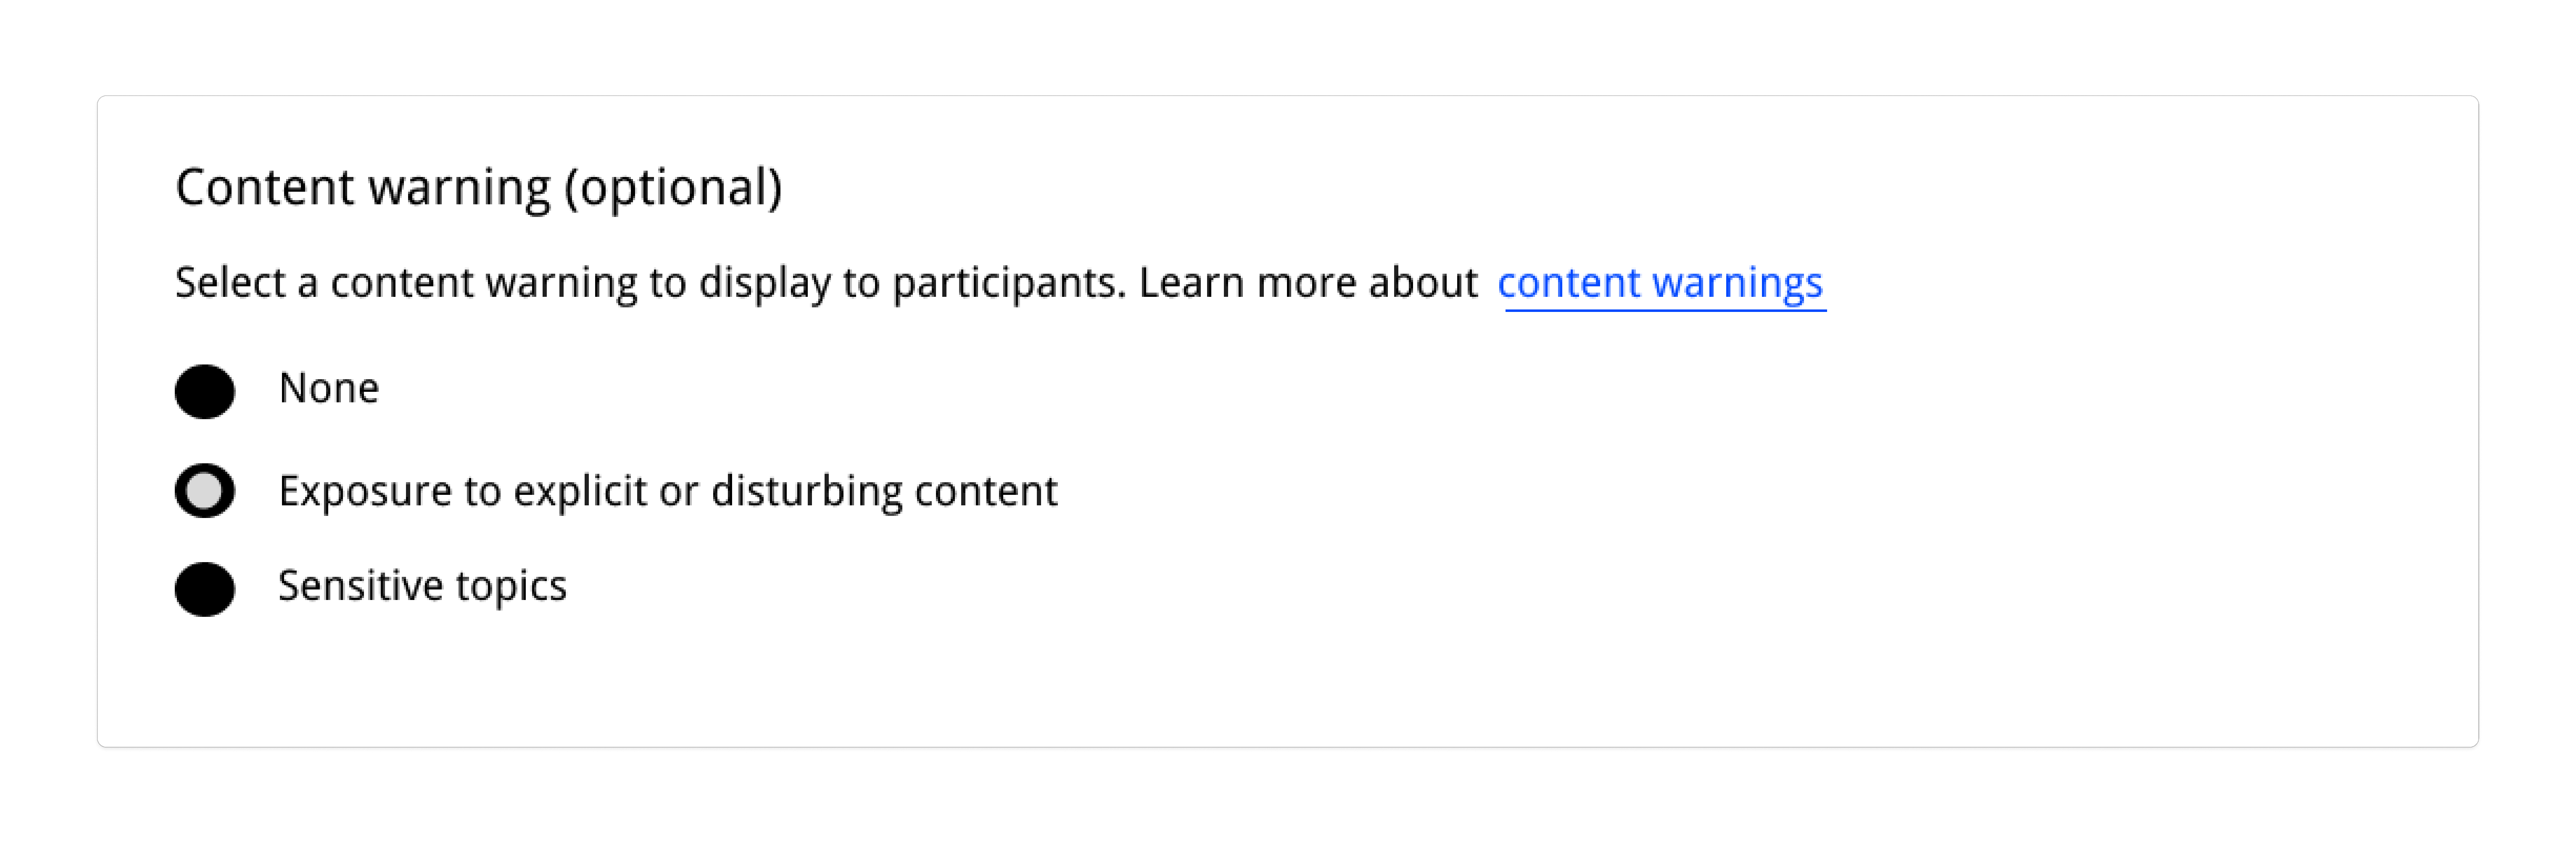
\includegraphics[width=\textwidth]{figures/study-probes/task-designer-probes/binary-task-designer.pdf}
        \caption{Binary}
        \label{fig:manual-binary}
    \end{subfigure}
    \hfill
    \begin{subfigure}[b]{0.48\textwidth}
        \centering
        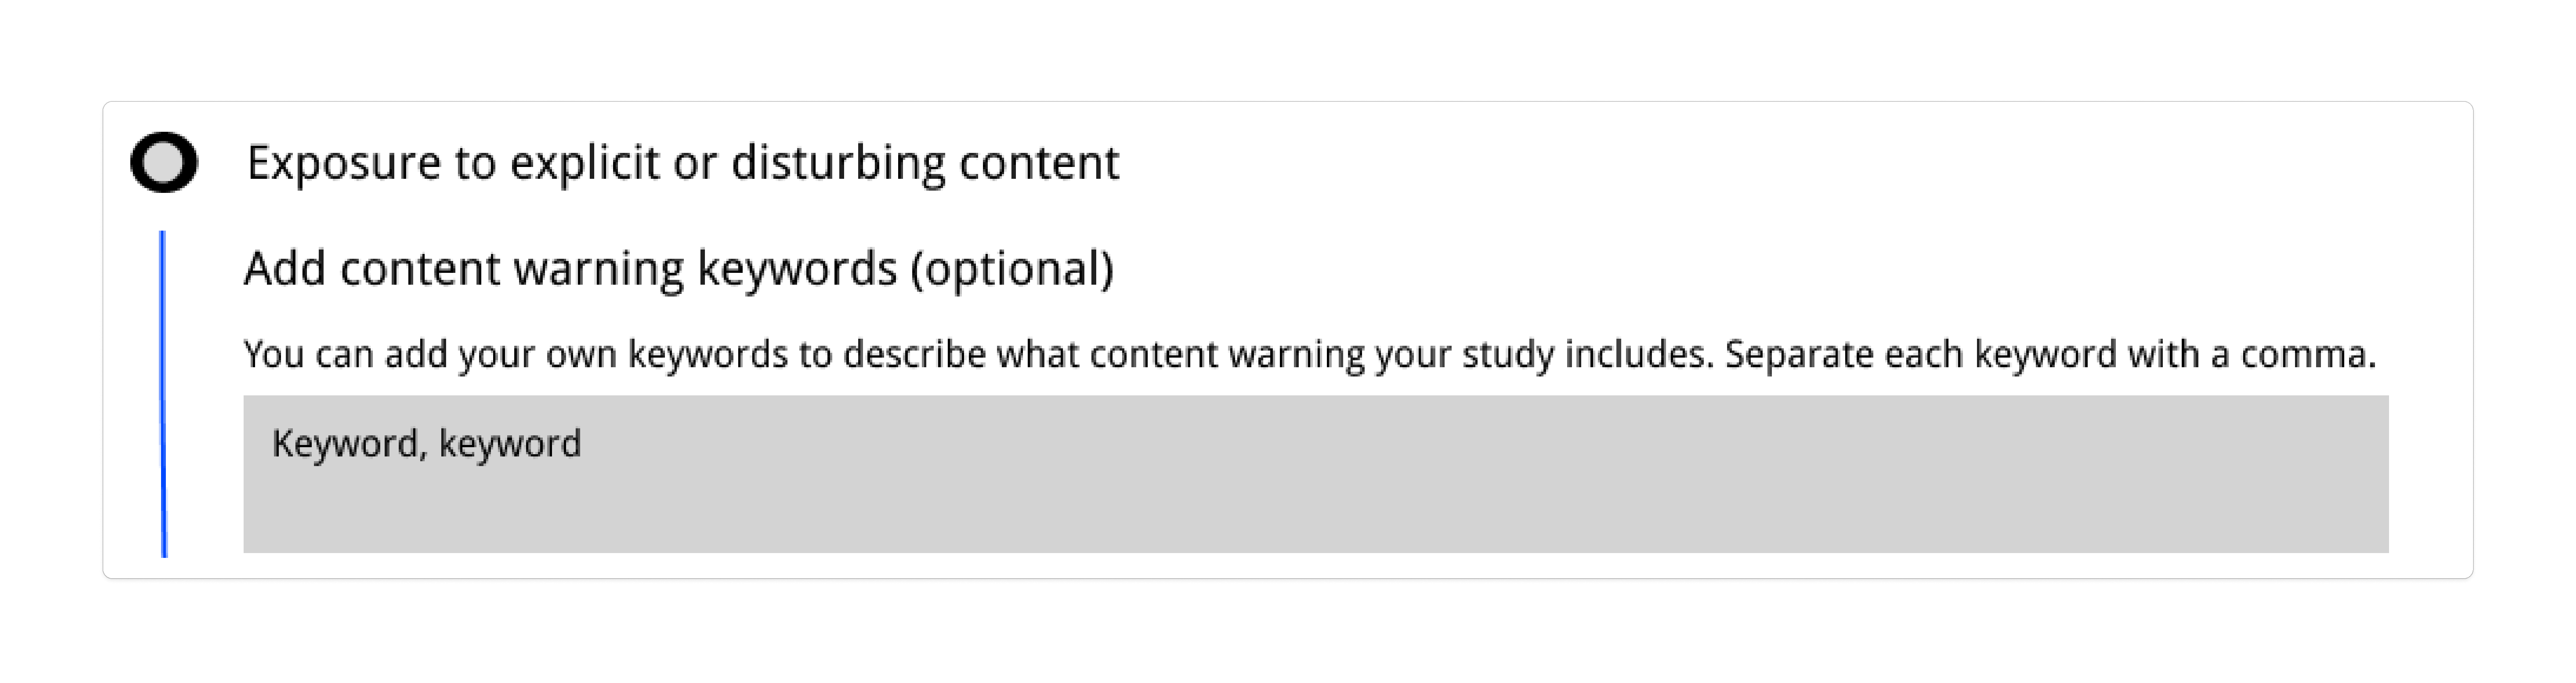
\includegraphics[width=\textwidth]{figures/study-probes/task-designer-probes/keywords-task-designer.pdf}
        \caption{(Keywords}
        \label{fig:manual-keywords}
    \end{subfigure}

    \vspace{0.5em}

    % Second row
    \begin{subfigure}[b]{0.48\textwidth}
        \centering
        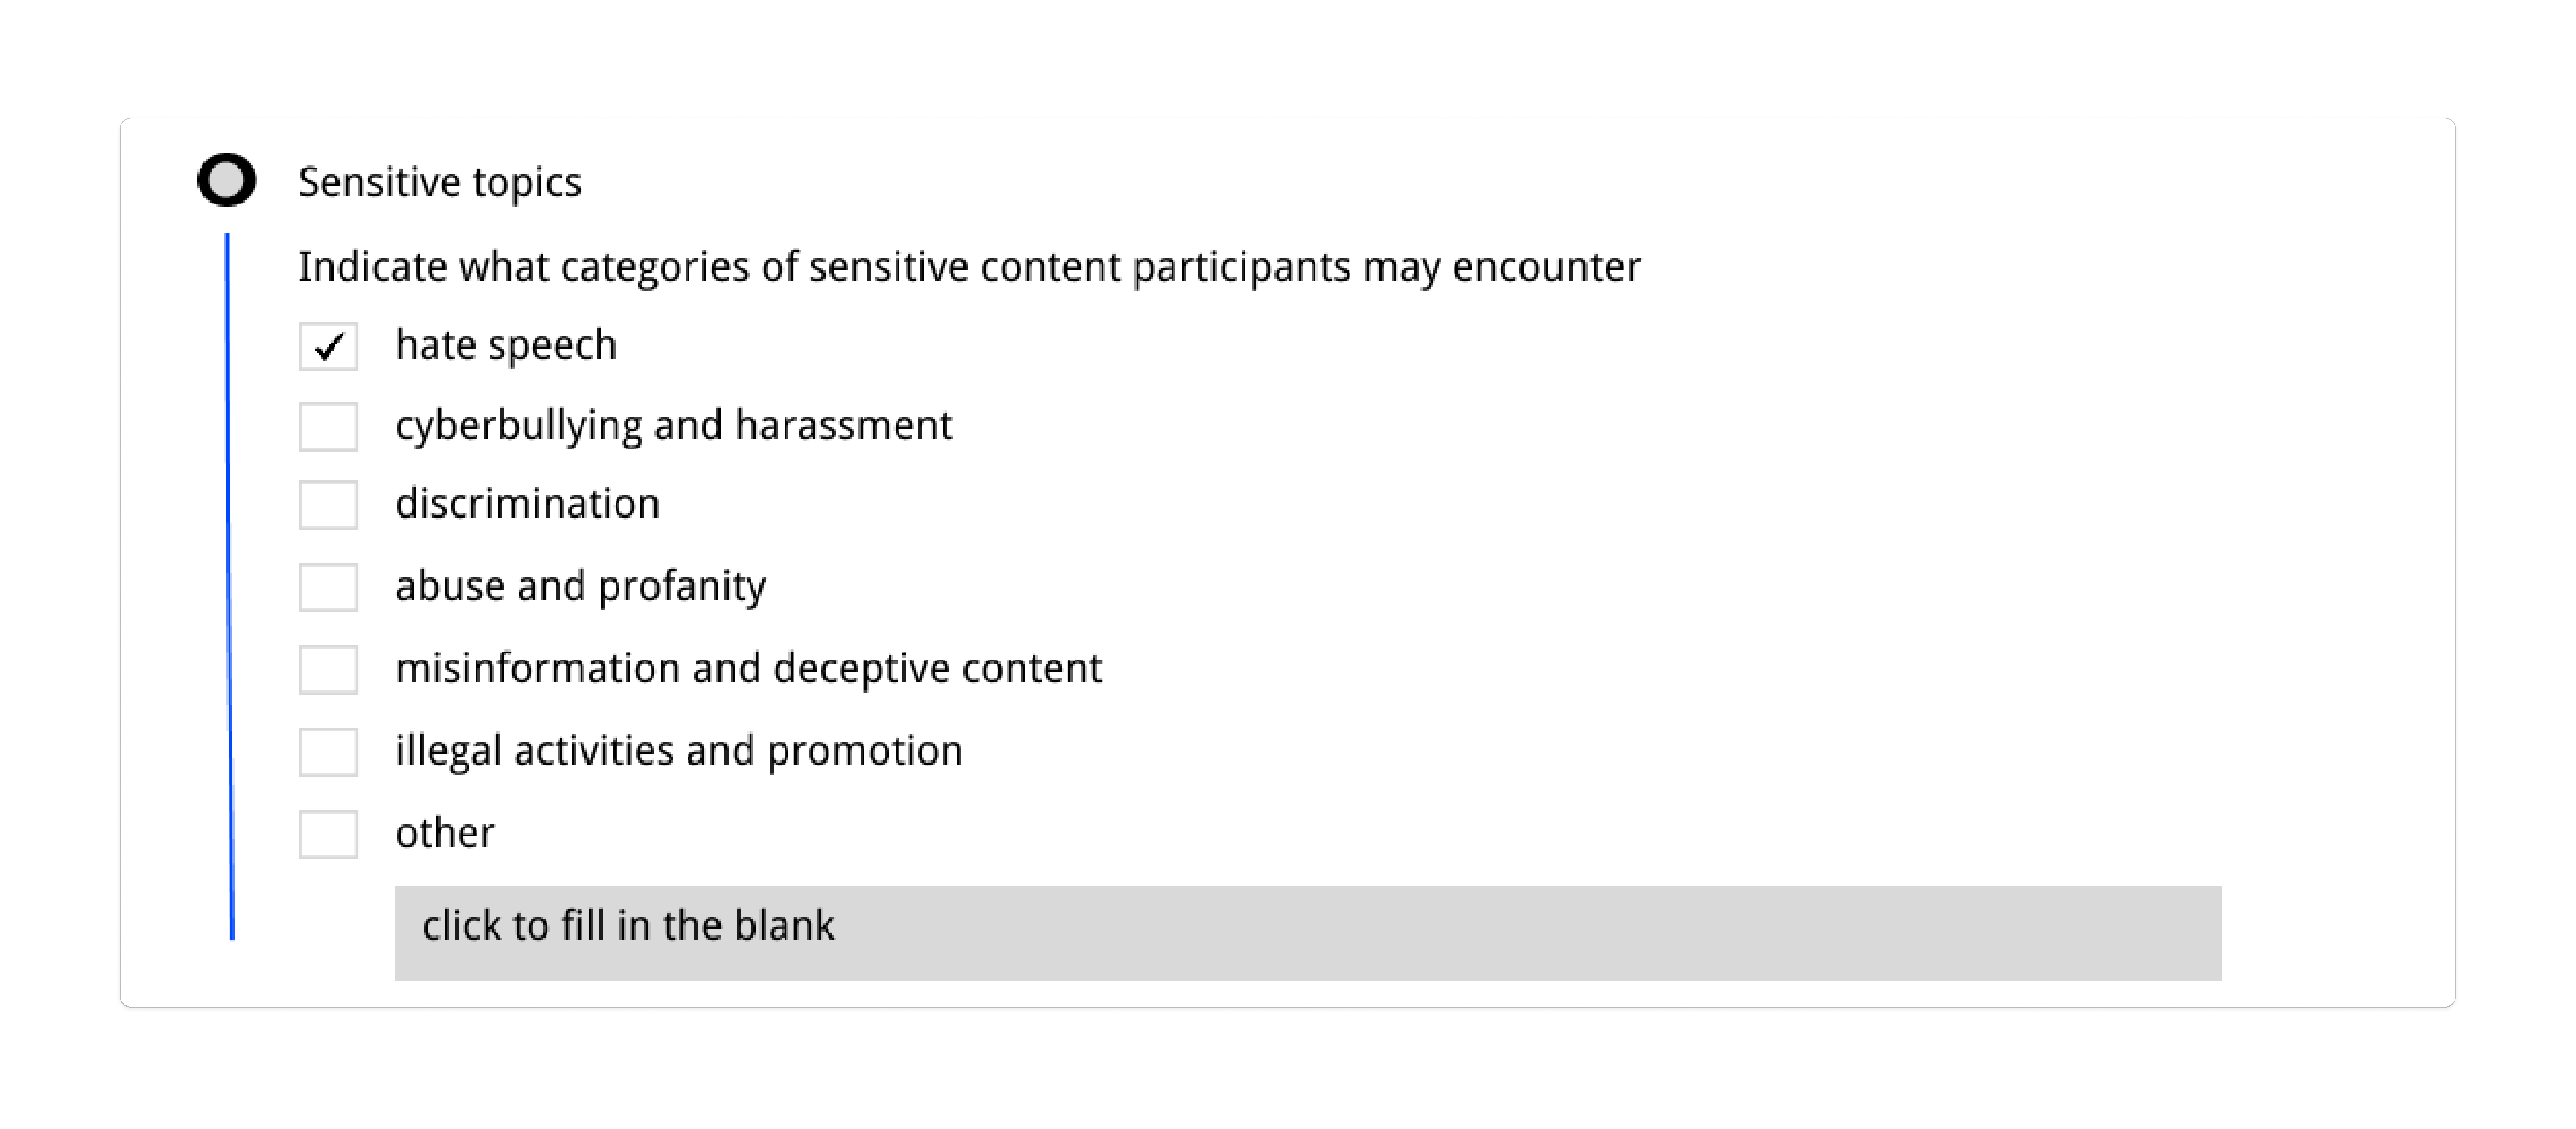
\includegraphics[width=\textwidth]{figures/study-probes/task-designer-probes/category-task-designer.pdf}
        \caption{Category}
        \label{fig:manual-category}
    \end{subfigure}
    \hfill
    \begin{subfigure}[b]{0.48\textwidth}
        \centering
        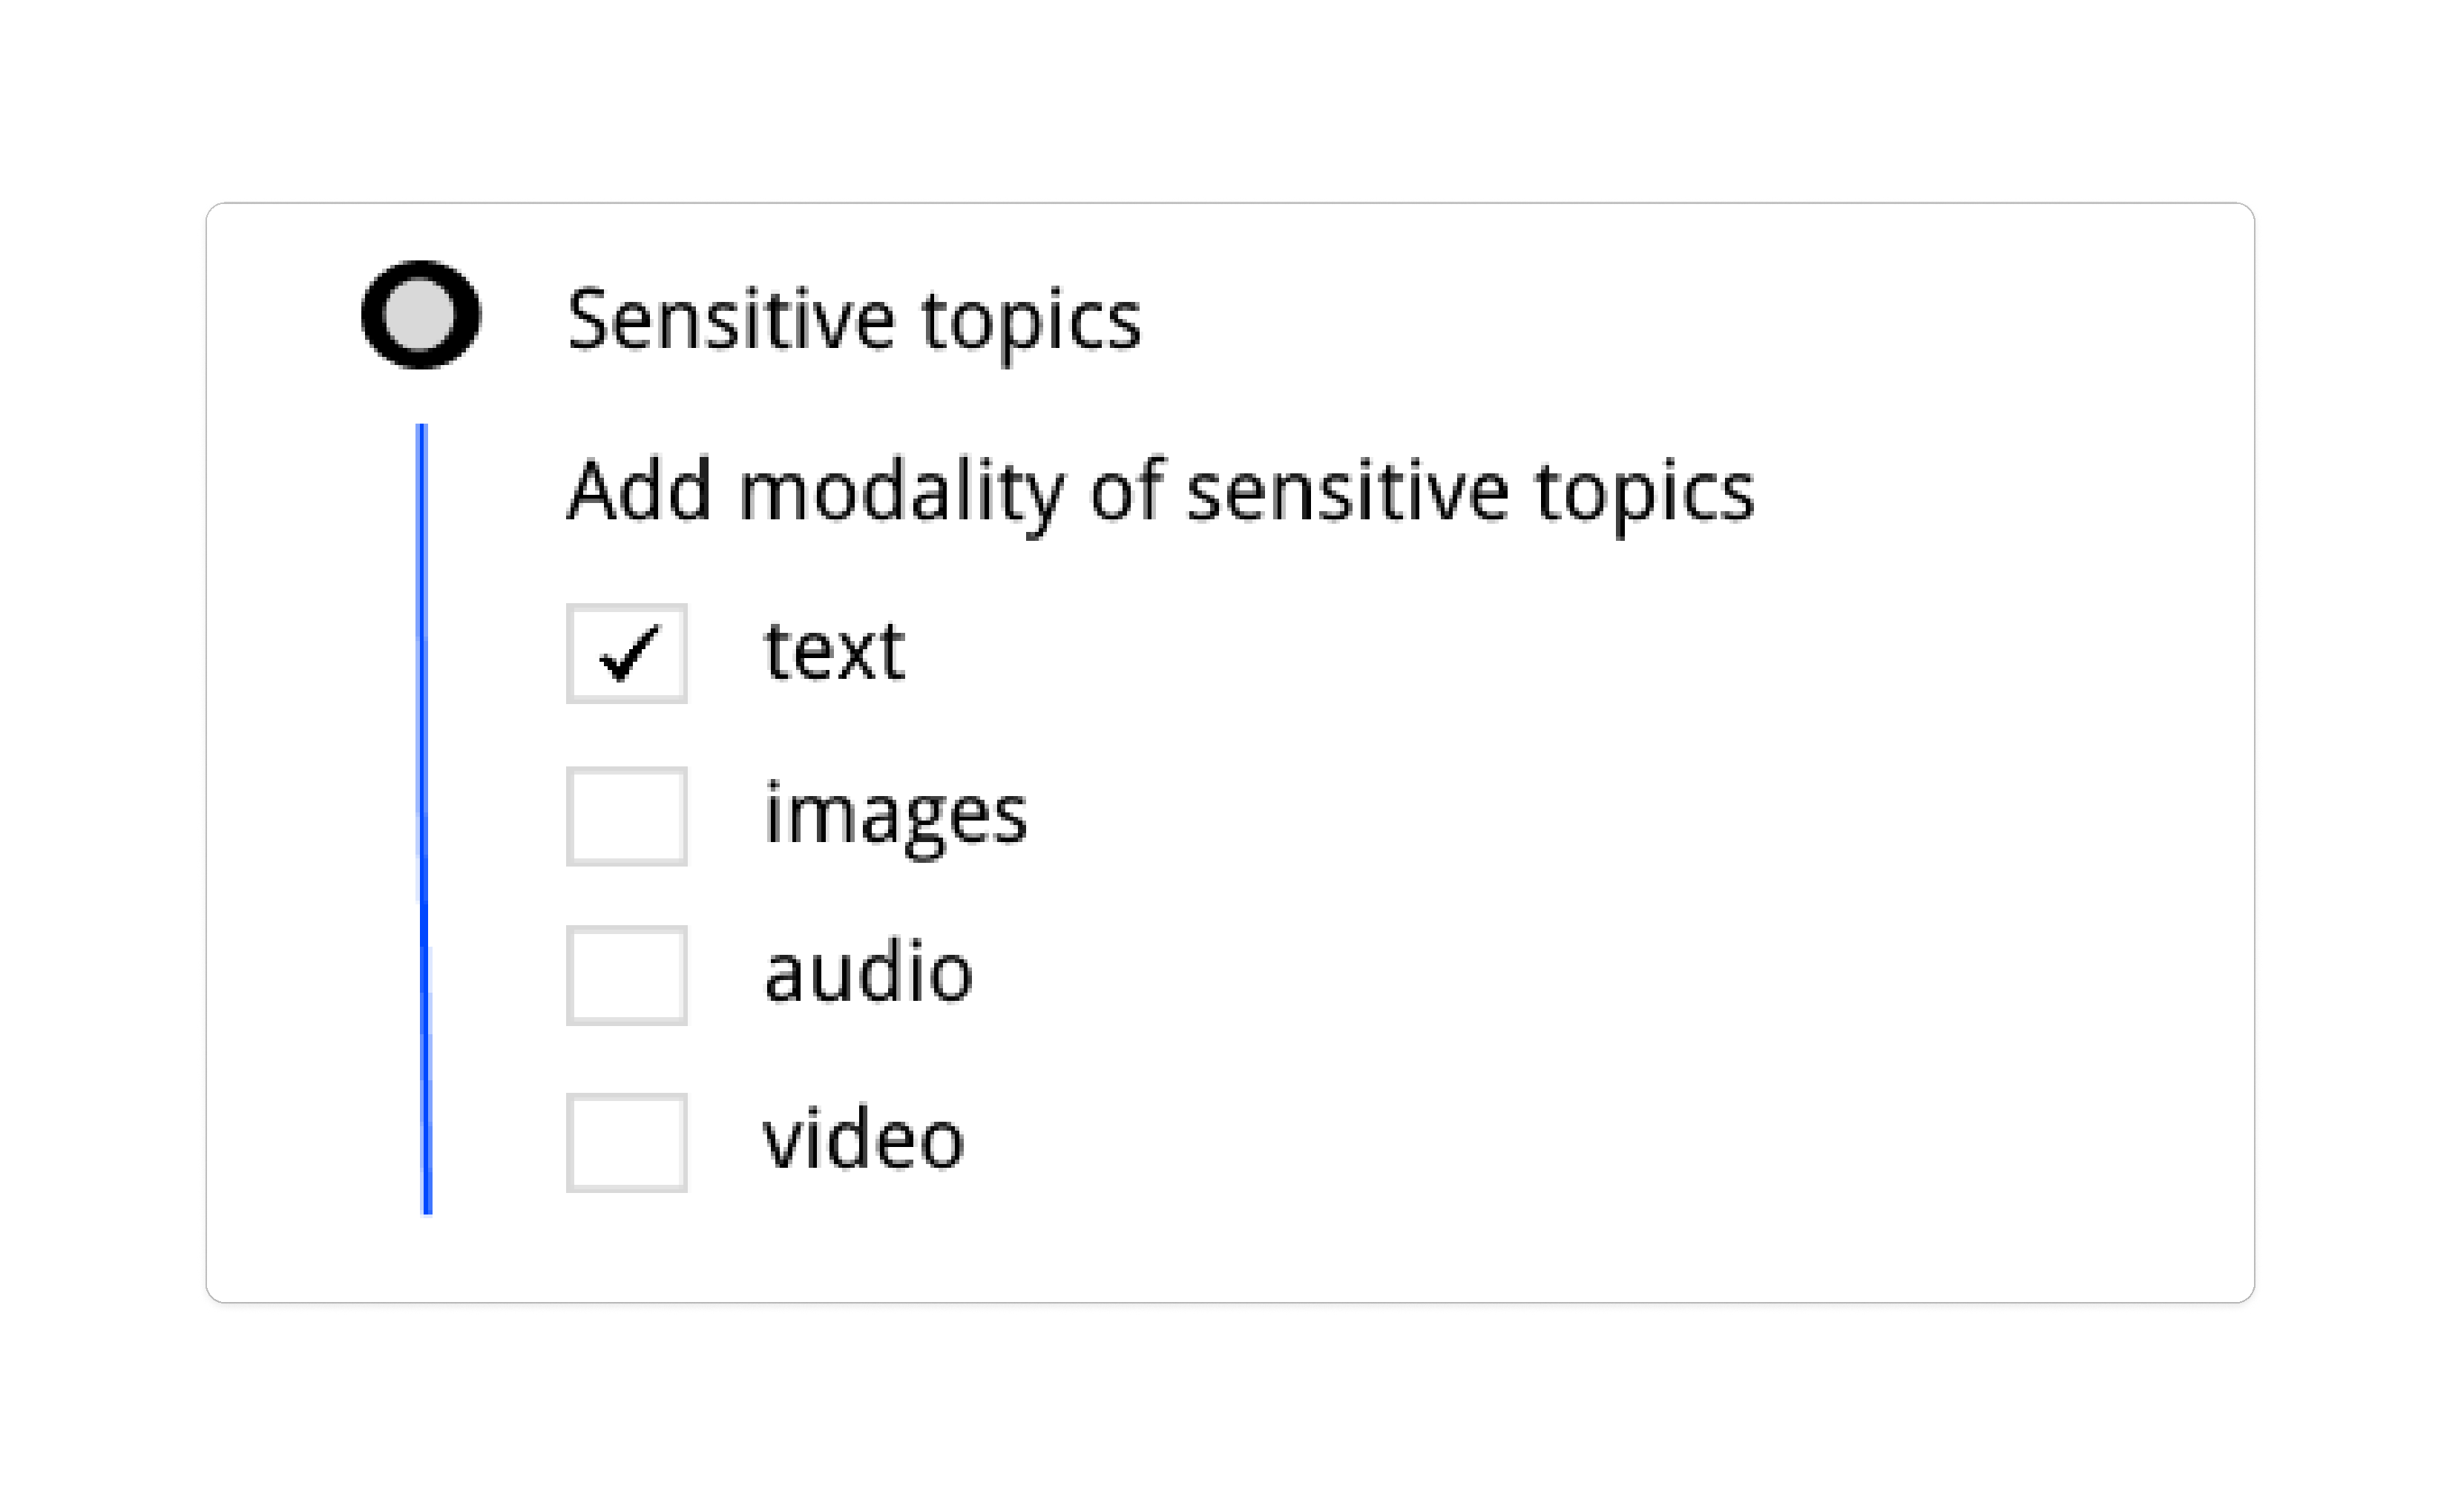
\includegraphics[width=\textwidth]{figures/study-probes/task-designer-probes/modality-task-designer.pdf}
        \caption{Modality}
        \label{fig:manual-modality}
    \end{subfigure}

    \vspace{0.5em}

    % Third row
    \begin{subfigure}[b]{0.48\textwidth}
        \centering
        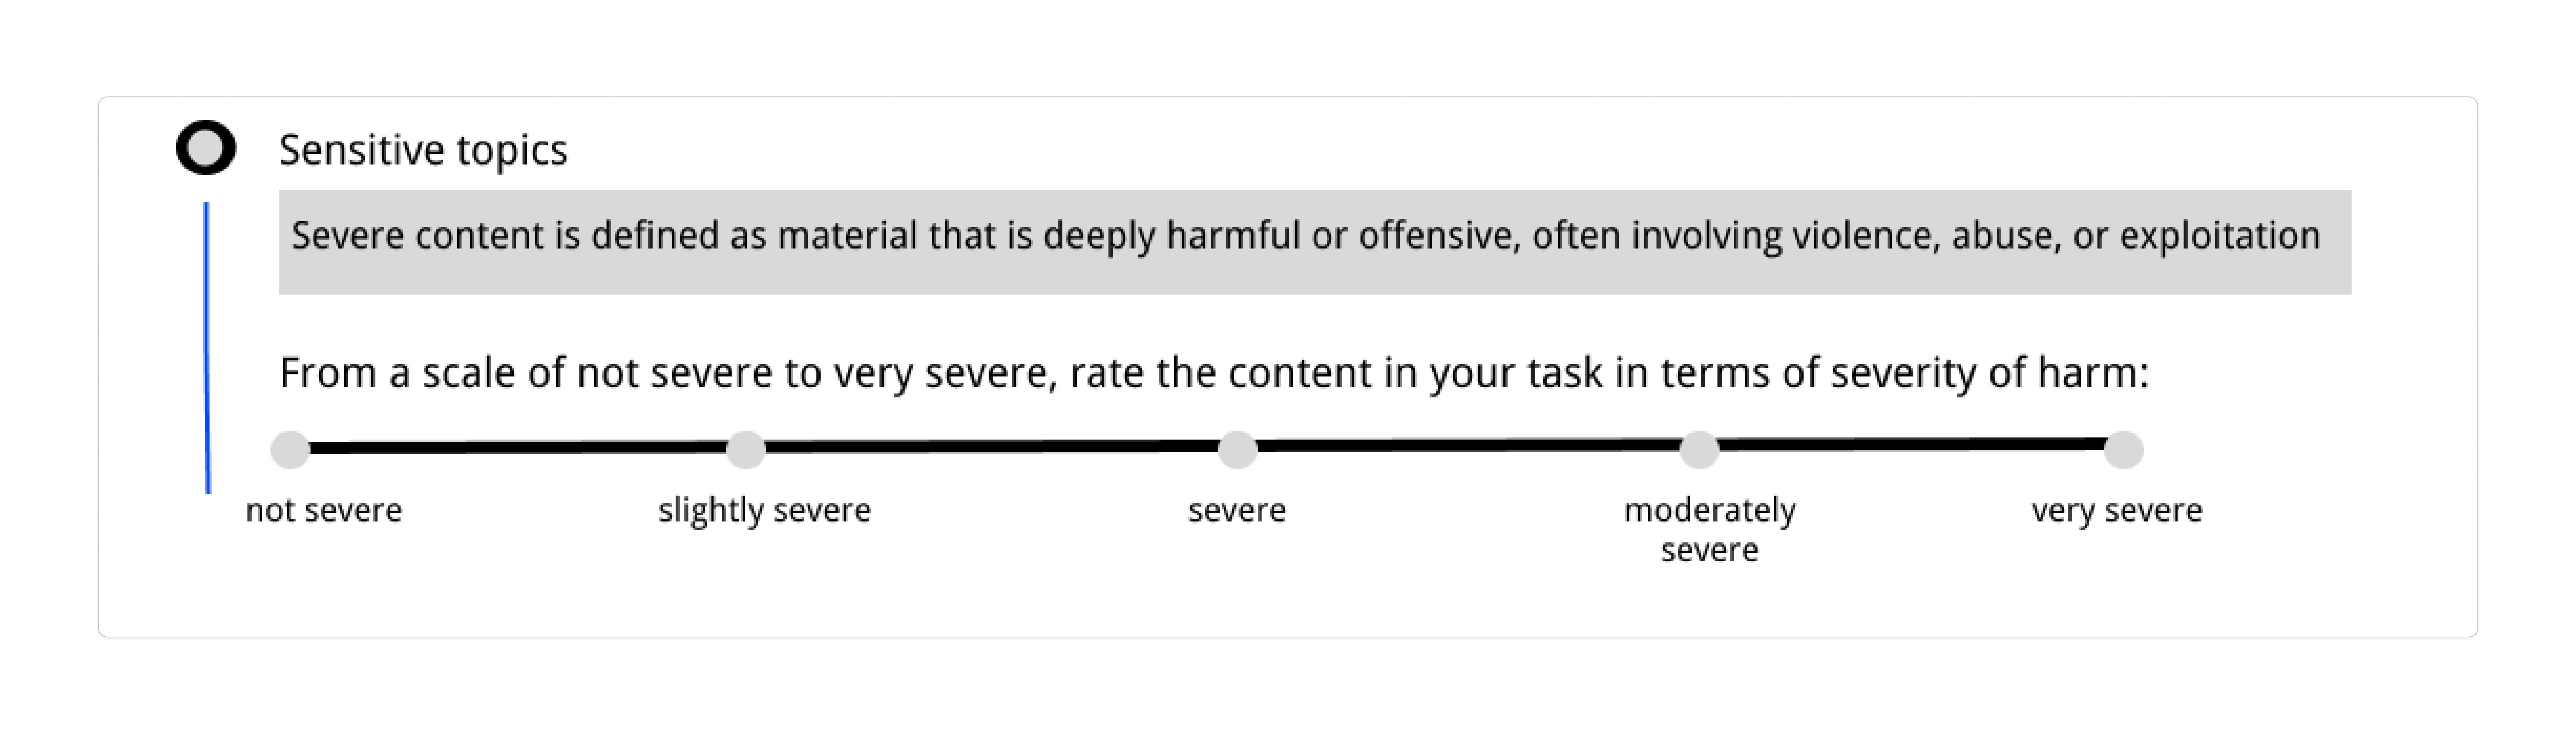
\includegraphics[width=\textwidth]{figures/study-probes/task-designer-probes/severity-task-designer.pdf}
        \caption{Severity}
        \label{fig:manual-severity}
    \end{subfigure}
    \hfill
    \begin{subfigure}[b]{0.48\textwidth}
        \centering
        
\includegraphics[width=\textwidth]{figures/study-probes/task-designer-probes/example-task-designer.pdf}
        \caption{Example}
        \label{fig:manual-example}
    \end{subfigure}
    \caption{Task designer manual options}
    \label{fig:task-designer-manual}
\end{figure}


\begin{figure}[htbp]
    \centering
    % Top row
    \begin{subfigure}[b]{0.48\textwidth}
        \centering
        \includegraphics[width=\textwidth]{figures/study-probes/AI-probes/AI-one-time.pdf}
        \caption{Generic AI suggestion\footnote{Icon credit: https://wallpapers-clan.com/sticker-png/cute-canary-bird}}
        \label{fig:AI-generic}
    \end{subfigure}
    \hfill
    \begin{subfigure}[b]{0.48\textwidth}
        \centering
        \includegraphics[width=\textwidth]{figures/study-probes/AI-probes/AI-explanation.pdf} 
        \caption{AI suggestion with explanation}
        \label{fig:AI-explanation}
    \end{subfigure}
    \vspace{1em} % Space between rows
    % Bottom row
    \begin{subfigure}[b]{0.48\textwidth}
        \centering
        \includegraphics[width=\textwidth]{figures/study-probes/AI-probes/AI-task-designers.pdf}
        \caption{Suggestion based on what other task designers have done}
        \label{fig:AI-based-on-others}
    \end{subfigure}
    \hfill
    \begin{subfigure}[b]{0.48\textwidth}
        \centering
        \includegraphics[width=\textwidth]{figures/study-probes/AI-probes/AI-workers.pdf} 
        \caption{Suggestion based on what workers have said}
        \label{AI-based-on-workers}
    \end{subfigure}
    \caption{AI warning suggestions}
    \label{fig:task-designer-AI}
\end{figure}

% challenge 
Another key tension we found was in task designers' desire for agency in determining how risk should be disclosed for these tasks, with workers' desire for accountability mechanisms to be in place to prevent instances of inadequate risk disclosure. Several participants who were task designers indicated that they wanted agency to make the final decisions about how to disclose risk in their tasks. As P1 explained: \textit{``I know everything about my research, and I want to explain my research by my word[s] and by myself''} (P1). Other participants were open to receiving additional support in determining what warnings were most appropriate for their tasks. When prompted about receiving AI and prediction-based suggestions, these participants expressed an optimistic outlook on using such tools. Several participants expressed that having some version of an AI suggestion for a warning would be helpful. Others explained that predictions based on ways other task designers disclosed risk (e.g., P3 and P12) as well as predictions based on what workers have indicated (e.g., P2) would help them (see Figure \ref{fig:AI-based-on-others}). Others emphasize that being able to receive quantitative recommendations \todo{add figure explaining the 90\% of other task designers added this warning option} would be particularly helpful and even persuade them to include a warning. As P3 explained:
\begin{quote}
    \textit{``I understand this [suggestion] is saying that [a warning will be placed by other task designers] about nine times out of ten. Then the possibility that that is going to happen is, you know, very high. And, you know, why would I go for the less likely than the most likely? So definitely, I'll go for the most likely.''} -P3
\end{quote}
As such, we surface a space for opportunities for further innovation and experimentation with the design of systems that may support ask designers in disclosing risk.

% suggestions
Despite some participants' optimistic views of tools that could support their risk disclosure process, the amount of agency that is afforded to participants who were task designers was a key point of contention. Some participants were happy to accept suggestions provided by the AI (e.g., P14), while others urged for the suggestions to guide risk disclosure with the task designer making the final decision. These participants proposed options such as having multiple suggestions to choose from (P2 and P3), an option to edit warnings rather than just accept suggestions (P7 and P11), and the integration of AI options into specific questions about risk disclosure, such as suggesting keywords for a warning (P7). 

Many of our participants were cautious about using such tools, illustrating specific challenges that may emerge when implementing such tools. P1 and P26 cautioned that a certain amount of trust in how the suggestion was formed--particularly if it was AI-based--was necessary for them. P26 in particular cautioned that the suggestion based on how other task designers have disclosed risk would not be helpful unless the suggestion can clearly explain how to calculates similarity between tasks: 
\begin{quote}
    \textit{``Without knowing what similar means, this is kind of vacuous. For example, I imagine the system in back end being like if the task involves the two modalities, images and text, then I compute a statistic on what are the labels being applied? Then if it's over 50\% I tell the user, X percent of similar tasks added a warning for X. This is type of broad statistics is just not useful, right? \dots Unless you have a very good idea [of what] similar really mean[s] and being able to tell what similar [means] feels like a pretty hard thing.''} -P26
\end{quote}
As such, we found that for several of our participants who were task designers, retaining agency to make final decisions on risk disclosure as well as being able to trust suggestions provided by an AI or otherwise recommendations were important considerations. 

From the worker perspective, there was a need for accountability in the case of failed or inadequate risk disclosure. Our participants who were workers expressed several different ideas on how accountability should be placed in this case. P21 expressed that it was the task designers' responsibility to provide an adequate warning and that they \textit{``should be held responsible for anything that comes up''} regarding their content warning (P21). Moreover, P21 also reasoned that platforms should enforce consequences for inadequate risk disclosure because it is the platform's job \textit{``to make their platform more [worker] friendly [so] everybody will be satisfied''} (P21). We observed that some of our participants who were task designers expressed a similar sentiment in agreement that platforms should be responsible for holding other task designers responsible for adequate risk disclosure (e.g., P2, P8, and P9). However, ideas on how platforms can implement mechanisms to first identify instances of inadequate risk disclosure brought up tensions with task designers' need for agency mentioned earlier. For instance, P17 proposed that platform review tasks after task designers enter information about their task. However, P1 expressed earlier that \textit{``regardless of the accuracy [of the AI review], I just have the fear or uncomfortable feeling about [being] scanned or judged''} (P1). While some participants, such as P26, argued that task designers concerned about worker well-being would not be bothered by platform review of how they disclose risks in their tasks, P1's concern illustrates a key tension in that task designers, uncomfortable with the mechanisms enforced on a platform, may go to another platform. \todo{better summary of this tension?} 

\subsection{Task Completion}

\subsubsection{Balancing task completion with freedom to stop}
Even after opting into a task, some participants who were workers described encountering unexpected harms or discomfort, raising tensions between the need for ongoing consent and the pressures of task completion that underpin platform and task designer goals.
Several participants who were workers explained reasons why they want the option to be able to stop a task due to being uncomfortable with exposure to content. For example, P16 said \textit{``I found some section of the task way too sensitive, which actually stressed me, but I had no option than to complete it. I wish there was that flexibility, that I could skip those parts''} (P16). Despite wanting the choice to stop a task after starting it, participants also described concerns about wanting to be compensated for their efforts or their worker accounts facing penalties. Some participants indicated they wanted at least partial payment for their effort, given they failed to complete the task because they were uncomfortable rather than any other reason (P18-P20). 
% quote from P18 about partial completion:  There are some percent that comes with making an attempt to reach a particular level to be paid. But like I said, if there is no means to communicate, I tell him your situation and how you could not further the whole thing, then anything that comes with it, you just have to just like it to end something, whether he pays you and as you just have to, like, accept it.

Moreover, P17 reasoned that regardless of compensation, they would prioritize their well-being, but also indicated they were concerned about receiving a penalty to their account:
\begin{quote}
    \textit{``if [completing the task] has a very high effect on your mental health, it doesn't matter for you to be paid or not. I don't really care if I'm paid or not. If I'm not comfortable with doing I'm not doing it. So that should be like the case, but it shouldn't have, like a penalty.''} -P17
\end{quote}

The idea of a partial payment model was something that some participants who were workers reported having positive experiences with (P18) and some participants who were task designers were receptive to. P26, who was a task designer, advocated that they wanted to still use data from a worker even if they didn't complete the task, explaining that partial compensation was reasonable in this case (P26). P18 proposed that the platform step in to enforce this type of model:
\begin{quote}
    \textit{``[The] platform should inform the [task designer] to to pay some amount of money, since it was stated that you're going to be getting [a specific] amount after completion \dots  because what [the task designer] say[s is] sensitive might not be actually what, what [I] perceive---like sensitive might be extreme to me, like very sensitive. So they should be able to compensate for that''} (P18)
\end{quote}
Thus, from needs advocated by both workers and task designers, a policy of partial payment for the case of RAI tasks may be a promising avenue to address this tension. 

\subsubsection{Fair pay for RAI content work}
The discussion of fair or adequate pay for not only crowdwork but RAI content work tasks specifically was another point of tension among our participants. Echoing calls for the establishment of fair payment to crowdworkers in prior literature~\cite{silberman2018responsible, irani2013turkopticon}, some participants who were workers expressed a desire for increased pay to do RAI content work tasks. In contrast, task designers and platform participants expressed concerns about budget limitations as well as payment being potentially coercive. 

Several participants who were workers indicated a desire to be paid at a higher rate, describing tasks they previously completed at pay rates close to what is the standard for U.S. minimum wage in several stages (e.g., \$12.50 USD an hour for P25). Examples were proposed ranging from \$30-\$50 USD (P15-P17 and P20). Many participants who were task designers were open to paying more for RAI content work tasks (e.g., P4 and P7). P14 proposed that platforms should charge 2-5\% more for such tasks. Some participants, like P4, were alright with paying a smaller percentage more only because they viewed it as a negligible increase in price. Other participants indicated that some judgment of whether their task had content that was `severe' enough to warrant charging a higher rate would be necessary (e.g., P9). For some of these task designers, paying a higher rate was also reasonable if they could access a population of workers who were more experienced doing RAI content work tasks, meaning that similar to the `AI taskers' on some platforms\footnote{https://participant-help.prolific.com/en/article/5baf0c}, these workers had a proven track record for successful completion of such tasks. From these task designers' perspectives, this meant they could both perform well on tasks and were able to deal with exposure to such tasks. (P7 and P14). 

However, the proposed model of partial payment was not without flaws. Many participants who were task designers expressed concerns that increasing payment for RAI content work tasks could unreasonably pressure workers to complete tasks that they may otherwise opt out of.  P9 described the problem: \textit{``all I'm saying is adding more money to those types of tasks would make people that are sensitive to some explicit or disturbing content to go ahead [and do them] without even looking back''} (P9). To counter this issue, P12 proposed that the increase in payment should not be publicized to workers, recommending that \textit{``it shouldn't be made public that they will be paid more for very severe tasks, because \dots [that] enhances the uncensored responses, where workers don't even pay attention to [the warning], since it is something they know that pays more''} (P12). Other task designers were not perceptive to the idea of increasing payment for RAI content work tasks simply due to the exposure to potentially harmful content (P3 and P10). These participants reasoned that, for example, it did not make sense to pay for tasks that take the same amount of time as other tasks (P10). For these participants, the appeal to the quality of worker responses was more compelling, as P3 stated they would be perceptive to paying more if the quality of worker responses was guaranteed (P3). On the platform side, participants who were platform representatives expressed a desire to better tailor incentives when possible to workers. For instance, P28 explained how they approach incentives:
\begin{quote}
    \textit{``If you are doing, like a red teaming event or some sort of, like data annotation thing for a very specific subset of people who might be participating in it, then the option for non-monetary awards is more beneficial because then you can, like, tailor your awards to those people's needs. Like, if we're doing something for college students we can be like `we'll give you five informational interviews and a glowing letter recommendation.' Whereas if you don't know your audience then money is the best option.''} -P28
\end{quote}
Overall, we surface tensions around how workers indicate a desire to be paid more for completing RAI content work tasks, while task designers have reservations about increasing payment in case it could negatively pressure workers. 


\subsection{Post-Task Completion}
\subsubsection{Encouraging quality feedback}
Finally, a challenge task designers and platform representatives described facing was that of collecting enough quality feedback from workers to gauge the effectiveness of their risk disclosure. 
Participants from all three populations described the importance of being able to provide and collect feedback about the effectiveness of risk disclosure for their tasks. Platform representative P27 reflected that it was difficult for them to collect feedback from workers even when presenting broad questions that were not targeted specifically to risk disclosure. Additionally, P27 also noted a need for more standardized practices for collecting feedback on their platform. For participants who were task designers, feedback was particularly helpful to gauge if the way risk was disclosed was effective or needed adjusting. For example, P11 illustrates a case where feedback would be helpful: 
\begin{quote}
    \textit{``Because [until] you get that feedback, and you don't actually know that this exact content can be very, very disturbing. Because you might think that it's just moderate, but you don't know that it's very, very severe and extremely disturbing''} -P11
\end{quote}
 For participants who were workers, feedback was described as one of the few places where workers could assert agency within the crowdsourcing process. P23 explained that after they complete a task \textit{``there's little I could do, but one thing I feel [is that] \dots after each task, you know you have a right [to be able to] leave a review. Leaving such review will make other other [workers] more aware of what was gonna [be in the task]''} (P23). Other participants expressed that feedback was an important outlet for them if they were hurt by the lack of risk disclosure, explaining their desire to complain or verbally \textit{``bash''} the task designer for their failure. Thus, we find that for many of our task designer and worker participants, feedback served as a crucial avenue of communication.

% need to add paragraph where it's not just feedback they want, but like nuanced, detailed feedback (which is so hard T_T)

When discussing how task designers could better attain feedback, both participants who were task designers and workers emphasized the need to respect worker agency in choosing to give feedback or not. Several task designer participants reasoned that not only was it a matter of free will because workers \textit{``should be able to choose things on their own free will''} (P13), but also that enforcing feedback may result in lower quality responses. Participants who were workers expressed a similar sentiment, with some emphasizing that they may be too tired or traumatized after a task to give feedback. P17 described an instance where they did not want to give feedback: \textit{``I was so stressed, like, I was so stressed that I just want[ed] to finish [the task] so I didn't give any feedback. [The task designer] asked for feedback. I just skipped it''} (P17). 

One of the solutions discussed to help task designers obtain feedback was to pay for it. P15, who was a worker, expressed that paying for feedback could help workers \textit{``take [their] time providing it''} (P15). Some participants who were task designers indicated they would be willing to pay workers for feedback, given its importance (e.g., P6 and P9). However, others stated they would not try to get feedback if they needed to pay for it (e.g., P5) or that if feedback was \textit{``just three clicks,''} (P12) it would be unnecessary to pay workers for it. Yet other participants cautioned that paying workers for feedback could result in \textit{``false feedback''} (P14) that was disingenuous. Overall, while there is potential in some design interventions that make feedback potentially easier to use for workers, we surface key challenges in collecting feedback, such as determining an appropriate model for compensation and ensuring the elicitation of nuanced feedback. 


\subsubsection{Mitigating harms from failed risk disclosure}
In instances where risk was not adequately disclosed to participants who were workers, some looked to task designers for acknowledgement or redress, but the absence of clear accountability structures encouraging such responses exposes a deeper tension between individual harm and diffusion of responsibility. Several participants who were workers felt it was important to receive a response from task designers when they raised problems with a task's  risk disclosure process (e.g., P15 and P17). Participants who had worked explained that responses from task designers helped validate the harm they experienced (e.g., P15 and P24). P22 explained that when task designers responded to their feedback it \textit{``makes me feel heard and sane at least. It tell sme that you actually value my opinion''} (P22). Moreover, some participants expressed that a receiving a response from a task designer reassured them that the task designer would want to improve their task's risk disclosure for future workers. P20 claimed that a response could \textit{``make me feel like the researcher understands how I feel and [is] willing to correct [the warning]''} (P20). 

Other participants struggled to envision the purpose of receiving a response that was not related to monetary compensation (P17 and P21). For instance, P17 stated they wanted to be able to contact a task designer \textit{``maybe we should be able to contact their company''} but struggled to envision what the task designer's organization could do other than provide compensation: \textit{``but the other thing I'm thinking about is, if I contact the company, what are they going to do about it?''} (P17). When asked about what they ideally wanted the task designer's organization to do, P17 stated \textit{``Oh compensate me, I guess''} (P17). Moreover, despite wanting compensation, P17 also acknowledged the potential for abuse of task designers' goodwill by other workers. 
% For example, P17 explained that the only thing a task designer could do is provide monetary compensation for the harm they experienced: 
% \begin{quote}
%     \textit{``I feel they should compensate me. That goes two ways, because some [workers] might misuse it. I just feel like they should compensate because they can't take away what I've seen. [What I've seen] still [stays] with me, so the only thing they can do is just compensate''} - P17
% \end{quote}
% In this reflection, P17 acknowledged the tension of workers potentially misusing task designers' goodwill, but still stands by their assertion that compensation is the only action task designers can take to remedy harm to them. 

Another suggestion that surfaced was for workers to receive resources for well-being. P27, who was a platform representative, suggested that platforms \textit{``offer resources. You can say like `if you experience issues, please reach out to [us]''} reasoning that if the platform is hosting such tasks \textit{``they should have a point of contact. The program manager, a mental health counselor, or something [else] in case people experience challenging issues in the work that they're doing''} (P27). Previously, P27's platform facilitated a red teaming task where they provided access to mental health professionals. In fact, prior research has established that particularly for some task designers who are academics, the practice of providing resources such as the phone number of link to a helpline has been commonly used~\cite{qian2025locating} \todo{add some papers about using these resources maybe along the line of like trigger warnings too}. When discussing their experiences receiving such resources, some of our participants who were workers felt strongly about how task designers and their organizations took responsibility in distributing such resources. For instance, for P17, task designers should provide helplines from their own company instead of pushing the responsibility to another party:
\begin{quote}
    \textit{``I think it's just [task designers] fulfilling [some] righteousness because obviously nobody's gonna call the number \dots because you're putting a task for people to do and you're asking them to call [another organization]. Is it [that organization] that gives [workers] the task? Doesn't make sense to me. You give [workers] a task. You should be the one offering [workers] like a helpline and all that.''} - P17
\end{quote}
P17's reflection highlights the complexity of such a space, indicating that the way in which task designers and platforms present resources could change how workers perceive how they are taking responsibility for remedying harm to workers. 

\section{Discussion}

% ideas I have
% opportunities for design/evaluation on crowdsourcing platforms and the need for this information to be widely shared
% parallels rai crowd workers are displaying compared to what's found in the literature --> the question of whether it's ethical to keep crowdsourcing in the future

\subsection{Design Implications}
% here we talk about specific design implications from the findings

\subsection{Negotiated Responsibility in Risk Disclosure}
% discussion of risk disclosure being a site of negotiated responsibility between our 3 groups. Our findings show how these actors hold different assumptions about who is responsible for identifying and mitigating harm. Acknowledging this dynamic allows us to shift our design question from how risk should be disclosed to who decides, when, and on what basis? 
Our study reveals that risk disclosure in AI data work is a socially negotiated process among workers, requesters, and platforms. We confirm previous work that found these groups hold distinct and at times conflicting assumptions about who should identify, assess, and communicate risks \cite{fieseler_unfairness_2019}. Workers often assume that task requesters or platforms have already vetted tasks for harm, while task designers may assume that workers bear responsibility for self-selecting out of sensitive content. Platforms, meanwhile, frequently promote a vision of shared responsibility while retaining control over infrastructure and moderation policies. These mismatches lead to practical gaps in risk disclosure and reinforce structural ambiguities around accountability \cite{Suchman2002LocatedAccountabilities, widder_dislocated_2023}.


This ambiguity invites us to reframe the design challenge. Rather than simply asking how risk should be disclosed, we must interrogate who decides, when, and on what basis. These questions draw attention to power asymmetries embedded in crowdsourcing platforms. Workers have limited opportunities to contest or shape disclosure practices, even as they bear the brunt of poorly disclosed risks. Task designers may want to warn workers, but are constrained by platform guidelines or unsure of what they are permitted to disclose. Platforms can offer guidelines or tools, but are often opaque about how risks are evaluated or escalated internally~\cite{roberts2019behind}.

By conceptualizing risk disclosure as a site of negotiated responsibility, we can open new design directions. Future tools might aim not just to standardize disclosure formats, but to mediate disagreement and dialogue across stakeholder boundaries \cite{fieseler_unfairness_2019}. For example, platforms could surface discrepancies in risk perception between task creators and workers, or allow workers to annotate disclosures with feedback. Designing for this kind of deliberation requires acknowledging that disclosure is a form of boundary crossing~\cite{Suchman2002LocatedAccountabilities}, not simply a transfer of information, but a process shaped by contested expertise, values, and institutional constraints.

Moreover, understanding these negotiations requires us to move beyond individualistic framings of responsibility. Instead, we can draw on theories of *distributed* or *relational* accountability, which emphasize how ethical obligations are produced through collective, situated practice~\todo{add citation on relational ethics or actor-network theory}. Such a lens complicates the assumption that risks can be fully known or managed in advance, and suggests the need for systems that are reflexive and adaptive over time.


\subsection{Beyond Risk Disclosure}
% where we can talk about workers needing more support (helpline isn't enough) and also what are platform gonna do if they provide a number of a product manager you can call? unrealistic?
While task-level risk disclosures are a critical starting point, they are only one component in a broader ecology of worker well-being. Our findings reveal that workers, even when appreciative of disclosure efforts, continue to face harm that is structural, cumulative, and poorly addressed by current platform support. Many participants described psychological strain from sustained exposure to distressing content, difficulty disengaging from harmful tasks, and a lack of avenues for recovery. Helplines and automated filters offer some relief, but fall short of meeting the scale and complexity of workers’ needs~\todo{add citation on emotional labor and crowdworker burnout}.

In particular, workers expressed a desire for more robust pre-task support. This includes not only clearer disclosures, but also access to training and reflection tools that could help them assess personal thresholds for harm and prepare emotionally for the work. Existing research on content moderation and trauma-informed design points to promising strategies here—such as onboarding experiences, harm typologies, and peer knowledge sharing—that could be adapted for the crowdsourcing context~\todo{add citation on moderation training or trauma-informed interface design}.

Post-task care is an even more underexplored frontier. Some workers suggested mechanisms such as debriefing spaces, access to mental health resources, or the ability to pause or escalate after encountering disturbing content. However, the logistics of such support remain unclear: who would provide it, under what funding model, and with what safeguards? In an industry defined by just-in-time labor and minimal worker protections, offering meaningful well-being resources challenges the very business models that platforms depend on~\cite{gray2019ghost}.

Moreover, the workers most vulnerable to psychological harm are often those with the least power to request accommodations. Crowdworkers span geographies, languages, and socioeconomic contexts—factors that mediate not only their exposure to harm but also their ability to access care. Designing for worker well-being thus requires a deeply intersectional approach, one that foregrounds structural inequalities rather than treating harm as a purely individual experience~\todo{add citation on intersectional HCI or global crowdwork}.

\subsection{Question of whether we should crowdsource RAI content work}
% cite implication to not design paper
% what type of task should be crowdsourced
% should be crowdsource at all
% can directly call out our limitation as a co-design study here, with power imbalance of workers
% from Hong this report has definitions of platform: https://www.ilo.org/sites/default/files/wcmsp5/groups/public/%40dgreports/%40dcomm/%40publ/documents/publication/wcms_645337.pdf
% - we focus on the complexities of this design space, but there is an itneresting question about whether it's effective or ethical to crowdsource this work
% - maybe we can crowdsource, but we don't make this into microtasks
% - in terms of what is effective, this does align with what our task designers want and some of our findings showed that some workers are open to this too
% - of course this will take away power from platforms
% - in terms of the ethics (cite literature) 
% this is sort of a policy implications section

Our findings also surface a deeper question: \textbf{Should we crowdsource risky or sensitive AI content work in the first place?} While our study focuses on improving the design of risk disclosures, it cannot sidestep broader concerns about whether the task environment itself is appropriate or just. As prior literature has shown, microtasking can fragment judgment, mask ethical complexity, and devalue the expertise required to make nuanced content decisions~\todo{add citation on fragmentation and judgment in crowd work}. These concerns are amplified in the context of RAI development, where annotation decisions can shape downstream system behavior.

Several task designers in our study justified crowdsourcing on the basis of diversity and scalability, noting that crowdworkers provide valuable perspectives and can be engaged more flexibly than full-time staff. Some workers echoed this, citing financial need or interest in meaningful participation. Yet the same workers also described feeling isolated, underpaid, and unsupported when engaging with emotionally fraught tasks. This suggests that current practices may extract value from worker insight without adequately compensating for the associated risks~\todo{add citation on labor extraction and affective value}.

Rather than rejecting crowdsourcing altogether, one alternative is to rethink how it is done. For example, longer-form or collaborative annotation formats might give workers greater context and control. Task structures could emphasize care and deliberation over speed, perhaps shifting away from performance-based incentives and toward reflective judgment. Some of these ideas mirror trends in community moderation or participatory research, where contributors are treated as co-creators rather than disposable labor~\todo{add citation on participatory AI or collaborative annotation}.

However, such changes would likely challenge platform logics and economic incentives. Implementing slower, more dialogic forms of labor requires reconfiguring not only interface design, but also compensation structures, labor policy, and institutional accountability. These are not merely technical or logistical challenges, but ethical ones. We therefore join prior scholars in calling for greater scrutiny of whether certain types of work should be crowdsourced at all—and under what conditions it can be considered just, humane, and sustainable~\todo{add citation on just data labor or AI ethics and labor}. 

\section{Conclusion}
The design space of risk disclosure in RAI content work is both essential and under-explored. As platforms increasingly allocate RAI content work tasks to crowdworkers, new mechanisms are urgently needed to ensure workers are not exposed to harmful content without, at the very least, having a robust consent process in place. While prior work has highlighted the importance of content warnings on social media platforms and disclosures for job contracts, far less attention has been paid to how these mechanisms function—or fail—in the context of outsourced labor for responsible AI development.  Our findings reveal the varied and often conflicting goals that shape risk disclosure in crowdsourced AI work. For instance, while task designers worry about scaring off workers with detailed warnings on tasks, workers seek clarity and autonomy in deciding what tasks to accept. Platforms, in turn, attempt to prioritize worker protection while meeting the needs of task designers and compliance with policies. We argue that any intervention in this space must contend with these competing logics. Rather than simplifying or flattening the problem, we advocate for systems that explicitly support negotiation, friction, and choice across stakeholders. Such approaches may offer more sustainable, transparent, and equitable models for risk communication---especially as AI development continues to rely on precarious and distributed forms of human expertise.





\bibliographystyle{ACM-Reference-Format}
\bibliography{_references, _references_aura, _references_crowdsourcing, _references_locating_risk}
% \input{sections/7_appendix}
\end{document}
\endinput


